\documentclass[12pt]{extarticle}
\usepackage[english]{babel}
\usepackage{NotesTeX}
%\usepackage{subfigure}
\usepackage{subcaption}
\usepackage{tikz}
\usetikzlibrary{arrows}
\usepackage{multirow}
\usepackage{listings}
\usepackage{extarrows}
\usepackage{parskip}
\usepackage{eurosym}
\usepackage{footmisc}
\def\code#1{\texttt{#1}}

\graphicspath{{../output/}}
\collaborationImg{
\includegraphics[width=30mm]{../../pictures/UIO.png}}

\author{\Large Vetle Nevland, Vetle Vikenes \& Sigurd Sørlie Rustad}
\title{\Huge Machine Learning: Bra Tittel}
\affiliation{\large FYS-STK4155 – Applied Data Analysis and Machine Learning
\\Autumn 2021\\Department of Physics\\University of Oslo\\\\\today}
\begin{document}
\abstract{This project investigates two numerical techniques for solving differential equations, forward euler and neural network. Conventional finite difference methods are efficient and accurate for solving not too intricate differential equations. Stability is an issue though, particularly for explicit schemes such as forward euler. Results from numerical simulations suggest that the output of a neural network is able to converge to the true solution. In contrast to forward euler, neural network is more or less unaffected by the time step. Instead, hyperparameters such as learning rate and epochs determine the accuracy and convergence property. Neural networks have their limitation of an extensive learning process, but offer a flexible and robust alternative to finite difference methods that is presumeably independent of temporal discretization. This opens for new possibilities in the field of differential equations. Our results strongly suggest that neural networks are well suited for simulating differential equations over long time periods, being much less sensitive of small time steps which would increase efficiency and accuracy simultaneously.}
\maketitle
\pagestyle{myplain}


\section*{To do}
\begin{itemize}
	\item NN: Skrive metode 
	\item NN: Finne beste NN (Resultater)
	\item Sammenlikne NN-FE feil og performance 
	\item Konklusjon 
\end{itemize}

\section{Introduction}

We will in no way answer all questions linked to the aforementioned methods. So that anyone can reproduce or continue our studies, we list all the code, results and instructions on running the code in our GitHub repository\footnote{\href{https://github.com/sigurdru/FYS-STK4155/tree/main/project2}{https://github.com/sigurdru/FYS-STK4155/tree/main/project3}}.

Neural network is a trending machine learning method due to its ability to solve a wide range of problems. By calculating the error at the output layer with an appropriate loss function, the weights and biases are updated accordingly to provide the best possible approximation to the true solution of the problem. The inner workings a neural network is considered a black box, difficult to justify theoretically, but its flexibility and wide applicability makes it a relevant method for approaching more unconventional tasks. This includes solving differential equations, which will be the main purpose for this project. 

The benefit of solving differential equations with neural network is that we don't need to know the analytical solution. By starting with a suitable guess of a solution, the neural network will converge towards the analytical solution given an appropriate loss function that initiaites gradient descent. Hence, neural networks are flexible enough to solve complex differential equations, including ODEs and PDEs. The focus in this project will be on solving a one dimensional diffusion equation. This is a PDE with a rather intricate analytical solution. It is of interest to investigate the potential for solving this PDE with a neural network.

A natural extension is to consider another differential equation with another applicablility. We will consider a first order ODE whose solution is the eigenvector corresponding to the largest eigenvalue of a real, symmetric matrix. Solving this differential equation will reveal the potential for a neural network to find eigenvalues of symmetric matrices. The result will be compared with traditional numerical methods for solving differential equations, particularly the forward euler method. A critical discussion of the methods will then be presented with focus on flexibility and computational efficiency. An overarching question considered is if neural networks can compete with state-of-the-art numerical methods for solving differential equations.


\section{Theory}
In the theory-section we aim to give a brief explanation of the main concepts and terminology used in this report. 

\subsection{The diffusion equation}

The full diffusion equation reads
\begin{equation}
\frac{\partial u(\mathbf{r}, t)}{\partial t} = \nabla \cdot \left[D(u, \mathbf{r})\nabla u(\mathbf{r}, t)\right],
\end{equation}
where $\mathbf{r}$ is a positional vector and $D(u,r)$ the collective diffusion coefficient. If $D(u,\mathbf{r}) = 1$ the equation simplifies to a linear differential equation
\begin{equation}
\frac{\partial u}{\partial t} = \nabla^2u(\mathbf{r}, t),
\end{equation}
or
\begin{equation}
\label{eq:diffusion_equation}
\left(\frac{\partial^2}{\partial x^2} + \frac{\partial^2}{\partial y^2} + \frac{\partial^2}{\partial z^2}\right) u(x,y,z,t) = \frac{\partial u(x,y,z,t)}{\partial t}
\end{equation}
in cartesian coordinates. In this report we are going to study a one dimensional rod of length $L=1$. I.e. we need the one dimensional diffusion equation
\begin{align}
\label{eq:diffusion_equation_1D}
\frac{\partial^2 u(x,t)}{\partial x^2} &= \frac{\partial u(x,t)}{\partial t},
\end{align}
with boundary conditions
\begin{align}
u(x,0) &= \sin(\pi x) \ \ 0\leq x\leq L,\\
u(0,t) &= 0 \ \ t\geq 0 \text{ and} \\
u(L,t) &= 0 \ \ t\geq 0.
\end{align}

\subsection{Analytical solution}


An analytical solution of the 1D diffusion equation can be dervied using the method of separation of variables.
For a complete derivation, please refer to the Appendix.
The analytical solution satisfying the given initial and boundary conditions is

\[ u(x,t) = e^{-\pi^2 t} \sin(\pi x) \]


\subsection{Explicit forward Euler}
In this section we want to cover the explicit forward Euler. By explicit we mean that the value at the next grid point is determined entirely by known or previously calculated values.

The one-dimensional diffusion equation \eqref{eq:diffusion_equation_1D} reads 
\begin{equation}
\frac{\partial^2u(x, t)}{\partial x^2} = \frac{\partial u(x,t)}{\partial t} \ \ \text{or} \ \ u_{xx} = u_t.
\end{equation}
In this report we are going to study a one dimensional rod of length $L=1$, with boundary conditions
\begin{align}
	u(x,0) &= \sin(\pi x) \ \ 0\leq x\leq L,\\
	u(0,t) &= 0 \ \ t\geq 0 \text{ and} \\
	u(L,t) &= 0 \ \ t\geq 0.
\end{align}

To approximate the solution, we have to discretize the position and time coordinates. We can choose  $\Delta x = L/N$ and $\Delta t$ as small steps in $x$-direction and time, respectively, where $N$ are the number of discretized points in $x$-direction. Then we can define the value domain of $t$ and $x$,
\begin{equation*}
t_j = j\Delta t, \ \ j\in \mathbb{N}_0 \ \ \wedge \ \ x_i = i\Delta x, \ \ \{i \in \mathbb{N}_0 | i \leq N\}.
\end{equation*}

The algorithm for explicit forward Euler in one dimension (from \cite{lectures2015} chapter 10.2.1) reads
\begin{equation}
\label{eq:forward_euler}
u_{i, j+1} = \alpha u_{i-1, j} + (1 - 2\alpha) u_{i,j} + \alpha u_{i+1, j}
\end{equation}
where
\begin{equation*}
\alpha = \frac{\Delta t}{\Delta x^2}.
\end{equation*}
This has a local approximate error of $O(\Delta t)$ and $O(\Delta x ^2)$. Experiments show that the following bound on $\alpha$ ensures stability.
\begin{equation}
	\label{eq:stability}
	\alpha = \frac{\Delta t}{\Delta x^2} \le \frac{1}{2}.
\end{equation} 

Even though $\alpha = 0.5$ is at the transition between stable and unstable solutions, experiments show that it is a safe choice for the diffusion equation that produces stable solutions \cite{Linge2017}. Thus, the stability factor $\alpha=0.5$ is used as default in this project. 

\section{Solving Differential equations with deep learning}
Many of the concepts we use in this section are covered in a previous report \cite{project2}. There, in the theory section, we cover central concepts like deep neural networks, cost functions, gradient descent, etc. In this report we will follow closely the work by Maziar Raissi et.al. \cite{raissi2017physics} and this Jupyter-Notebook\footnote{\texttt{https://colab.research.google.com/github/janblechschmidt/PDEsByNNs/blob/main/PINN \_Solver.ipynb\#scrollTo=1PlqQM9aZEkd}}. This method works with any partial differential equation (PDE), however for simplicity we will look at the diffusion equation in one dimension \eqref{eq:diffusion_equation_1D}. 

The idea is that we have some neural network $N$ with parameters $\theta$, including $x$ and $t$ as inputs, which returns $u_{\theta}(x,t)$. After training the neural network, one obtains the parameters $\hat{\theta}$ that best approximates its output with the actual solution, $u(x,t)$, of the PDE
\begin{align*}
	u_{\hat{\theta}} (x, t) \approx u(x, t).
\end{align*}

The process starts by defining a trial function $u_{\theta}(x,t)$ which is an initial guess of the actual solution $u(x,y)$, defined as

\begin{align}
	u_{\theta}(x,t) = u_0(x, t) + f\big(x, N(x,\theta)\big),
	\label{eq:NN_model}
\end{align}
where $u_0$ is a function specifically designed to satisfy the initial and boundary conditions of the PDE. The function $f$ is the part that is to be optimized by the algorithm. It depends on $x$ and the parameters $\theta$ through the neural network $N$, and should return 0 for the initial and boundary conditions. Constructing the function $f$ should beneficially incorporate prior knowledge about how the solution behaves, because this will accelerate the learning process.

\par We then define the residual $r_\theta(t, x)$, which is the output of the neural network inserted back into the PDE \eqref{eq:diffusion_equation_1D}
\begin{align}
	r_\theta(x, t) \equiv \frac{\partial u_\theta}{\partial t} - \frac{\partial^2 u_\theta}{\partial x^2}.
	\label{eq:residual}
\end{align}

Ideally this should be zero, impying a perfect reproduction of the actual solution. The residual becomes our main object for training, as it gives a measure of how good the neural network approximates the actual solution. For the neural network to improve its predictions a loss function is required, which is to minimized. For this we use the mean sum of squared residuals, including the initial and boundary points, across all data samples $n$. 

\begin{align*}
	L(x, t, \theta) = \frac{1}{n} \sum_{i=1}^n [r_\theta(x_i,t_i)]^2 + \frac{1}{n_B}\sum_{i=1}^{n_B} (u_{\theta}(x_b,t_i) - u(x_b,t_i))^2 + \frac{1}{n_I} \sum_{i=1}^{n_I} (u_{\theta}(x_i,0) - u(x_i,0))^2,
\end{align*}
where $n_B$ and $n_I$ is the number of training points on the boundary and the initial time step, respectively. Boundary points are given by $x_b$.
Optimization is then done through gradient descent, minimizing the loss with respect to the parameters $\theta$

\begin{align*}
	\theta \leftarrow \theta - \eta \nabla_{\theta}L(x,t,\theta),
\end{align*}

where $\eta$ is the learning rate, which can either be constant or variable, depending on the optimization strategy.
The loss function converges towards zero for the optimal parameters $\theta$, in which case the gradient of the loss function vanishes. As a result, the parameters will hardly update anymore through gradient descent, indicating that we have reached an optimal solution.


\subsection{Solving eigenvalue problems}
Deep neural networks are capable of solving more or less any differential equation. We will in this section follow the work of Yi et. al. (2004) \cite{yi2004neural} closely, using the same first ODE as them and closely following their methods for finding the eigenvalues. The first order ODE in question is given as     
\begin{equation}
	\frac{dx(t)}{dt} = -x(t) + f[x(t)],
	\label{eq:diff_eig}
\end{equation}
where
\[ f(x) = [x^TxA + (1 - x^TAx)I]x \]
where $A$ is a real symmetric matrix of shape $(n\times n)$ and $t \ge 0$ represents time. The solution of the neural network is given by $x(t)$ with dimensions $(n_t\times n)$, where $n_t$ is the number of time steps. The ODE \eqref{eq:diff_eig} is applicable for finding the eigenvalues of $A$. An equilibrium point $\tilde{x}$ of a differential equation is a solution that is stationary, that is a state where the solution doesn't change anymore, mathematically expressed as $\frac{dx}{dt} = 0$. It can be shown that the equilibrium points of \eqref{eq:diff_eig} span the eigenspace of $A$, implying that the equilibrium points are precisely the eigenvectors of $A$. That is, any $\tilde{x}$ that satisfies
\begin{align*}
	\frac{d\tilde{x}(t)}{dt} &= -\tilde{x} + f[\tilde{x}(t)] \\
	&= -\tilde{x} + [\tilde{x}^T\tilde{x}A + (1 - \tilde{x}^TA\tilde{x})I]\tilde{x} \\
	&= \tilde{x}^T\tilde{x}A\tilde{x} - \tilde{x}^TA\tilde{x}\tilde{x} = 0
\end{align*}
is an eigenvector of $A$. The rayleigh quotient formula can then be used to find the corresponding eigenvalue, given by
\begin{align} \label{eq:rayleigh_quotient}
	r = \frac{\tilde{x}^T\tilde{x}}{\tilde{x}^T A \tilde{x}}
\end{align}

An essential question is how the neural network should be initialized. That is, what trial solution of the form \eqref{eq:NN_model} should be chosen? Convergence analysis reveal that any non-zero trial solution $x(0) \in \mathcal{R}^n$ will give a solution of \eqref{eq:diff_eig} that converges to an eigenvector of $A$. Moreover, if $x(0)$ is not orthogonal to the subspace spanned by the largest eigenvector $\lambda_{\mathrm{max}}$ of $A$, then the solution $x(t)$ converges to an eigenvector corresponding to $\lambda_{\mathrm{max}}$.

The differential equation \eqref{eq:diff_eig} is a first order nonlinear ODE. Generally, solving a nonlinear differential equation numerically is a comprehensive process involving discretization in time followed by linearization through an iterative method (e.g Newton's method). Explicit schemes are an exception though, as all nonlinear terms are of the previous time step, hence are known. This allow us to easily solve \eqref{eq:diff_eig} numerically using the forward euler method. Discretizing the equation and solving for next time step $n+1$ gives

\begin{align*}
	\frac{x^{n+1}-x^n}{\Delta t} &= -x^n + f[x^n] \\
	\frac{x^{n+1}-x^n}{\Delta t} &= (x^n)^T x^n A x^n - (x^n)^T A x^n x^n \\
	x^{n+1} &= x^n + \Delta t\big[ (x^n)^T x^n A x^n - (x^n)^T A x^n x^n \big]
\end{align*}

Starting with a non-zero initial condition $x^0 = I(x)$, iteration over time steps will make the subsequent solutions converge towards the eigenvector corresponding to the largest eigenvalue of $A$, as long as the forward euler scheme is stable. The stability criteria depends on the discretization parameter $\Delta t$, and is to be approximated empirically. 



\section{Method}
\subsection*{Unit testing}

Before the numerical explicit scheme is applied to a particular problem, it is important to test that the discretized equations return expected results. Unit tests are constructed to test the implementation. This is done by manually calculating the solution of the first two time steps given the initial condition, and comparing the result with that obtained by the numerical scheme. Since the same recursive formula is used for all time steps, it is sufficient to test the two first time steps. To avoid too much computations we choose five equally sized intervals between $x=0$ and $x=L=1$, that is $\Delta x = 0.2$. The time step is set to $\Delta t = 0.01$, ensuring stability.
For time step $j$, that is $t=j\Delta t$, we have the following two boundary values and four interior points

\begin{align*}
	u_0^1 &= u_5^1 = 0 \\
	u_i^1 &= \frac{\Delta t}{\Delta x^2}u_{i+1}^0 + (1 - 2\frac{\Delta t}{\Delta x^2})u_i^0 + \frac{\Delta t}{\Delta x^2}u_{i-1}^0 \\
	&= 0.05u_{i+1}^0 + 0.9u_i^0 + 0.05u_{i-1}^0
\end{align*}

The initial condition used is $u_*^0 = \big(\sin(0),\:\sin(0.2\pi),\:\sin(0.4\pi),\:\sin(0.6\pi), \:\sin(0.8\pi),\:\sin(\pi)\big)$. If the results of the code match those manually calculated up to machine precision, it verifies the internal functionality of our implementation of forward euler. The results of the unit test are provided in Table \ref{tab:unit_test} in Appendix.



\subsection{Neural network setup}
\textcolor{red}{Sigurd: Skriv hvordan du setter opp neural network her. Skriv også hva du kommer til å teste (dybde) og hva du ikke skal teste.}

\textcolor{red}{Vetle og Vetle tenker at det er fint å bruke loss for å finne beste NN, og når det er funnet så regner vi ut MSE o.l. med metoden under for sammenlikning.}

\subsection{Accuracy assessment}
The unit test shows that the forward euler scheme works as expected, but to what accuracy can it reproduce the analytical solution and how does it compare to the neural network? To address these questions we will present some concrete methods for studying the solvers.

As discussed in the theory section, following equation \eqref{eq:stability}, $\alpha=0.5$ produce stable solutions for the diffusion equation. Throughout this report we will therefore use a time step of $\Delta t = \alpha \Delta x^2 = 0.5\cdot \Delta x^2$ for different choices of spatial resolution, and not consider other stability factors. We will limit our study to two spatial resolutions, namely $\Delta x = 0.1$ and $\Delta x = 0.01$.  

The first analysis we perform is the time evolution of the mean squared error (MSE) of the forward Euler solution. The MSE at a given time step, $j$, is given as 
\begin{align} \label{eq:MSE}
	\mathrm{MSE_j} = \frac{1}{N}\sum_{i=0}^N (u_i^j - u_{e,i}^j)^2 
\end{align}
where $u_e$ denotes the analytical solution. We expect the MSE to be zero initially, as numerical solution for the first time step is simply the initial condition. Proceeding, we expect an increasing MSE up to a certain point. Our boundary conditions results in the diffusion equation approaching $u(x,t)=0$ as $t$ increases, causing the MSE to eventually decline after a certain time. Combined with the unit tests, this serves as a simple method of validating our result.  
\textcolor{red}{Skal vi plotte dette for NN også?}

To proceed, we will study the solutions at two different times, $t_1$ and $t_2$ for both $\Delta x = 0.1$ and $\Delta x = 0.01$. We choose $t_1=0.1$ and $t_2=0.5$, where $u(x,t_1)$ is significantly curved and $u(x,t_2)$ is almost linear. These times will serve as the foundation for comparing the performance of our explicit numerical solver to that of the neural network. With the forementioned time periods and spatial resolutions, we compare the MSE of the two models, using equation \eqref{eq:MSE}. 

As a final study, we would like to plot the absolute difference between the numerical solutions and the analytical one for both $t_1$ and $t_2$. 
\begin{align} \label{eq:absolute_difference}
	\Delta u_i^n = u_i^n - u_{e,i}^n
\end{align}
Our main purpose of this is to see whether the neural network can circumvent one of the major drawbacks of the forward Euler scheme, namely the error caused by the discrete time steps advancing the solution more than it should. Solving the diffusion equation with forward Euler, we expect equation \eqref{eq:absolute_difference} to yield a negatively curved plot, with the boundaries being zero and the largest error occuring at $x=L/2$. This is due to the discretized solver advancing the solution by too much at each time step, affecting the succeeding calculations throughout the simulation. The biased error of the forward Euler scheme will cause big problems for more complex differential equations, where solutions don't converge to a stationary state. One major advantage of using neural networks will thus be if it yields unbiased errors that doesn't propagate throughout the simulation. \textcolor{red}{Kanskje litt dårlig forklart over, så skriv gjerne om}



\subsection{Finding eigenvalues}
Using the neural network model \eqref{eq:diff_eig} to find the eigenvalues of a real, symmetric matrix $A$ requires a trial solution \eqref{eq:NN_model} to initiate the network. The trial solution must fulfill the convergence property to guarantee that we end up with the eigenvalues. Hence, we define the initial condition $x_0 \in \mathcal{R}^n$ to be a vector of randomly generated numbers between zero and one. Since we don't know the eigenspace corresponding to the largest eigenvalue a priori, we have no guarantee that the trial solution is not orthogonal to the eigenspace corresponding to the largest eigenvalue. The probability of non-orthogonality, though, can be increased by adding random perturbations.

Even though a non-zero trial solution is the only requirement for convergence, there are strategies for improving the \textit{rate} of convergence. If we have some idea or preknowledge of a solution of the differential equation, incorporating this in the trial solution helps accelerate the learning of the neural network. The ODE \eqref{eq:diff_eig} is of first order with a term involving $\frac{dx}{dt}$ on one side and a term involving $x$ on the other. This is reminiscent of an exponential solution. Therefore, a smart initialization strategy of \eqref{eq:NN_model} is 

\begin{align*}
	g_{\theta}(t) &= g_0(x(t)) + f[x(t),N(x, \theta)] \\
	&= e^{-t}x_0 + (1 - e^{-t})N(x(t), \theta)
\end{align*}

This expression fulfills the condition of a trial solution, namely that it must return the initial condition $x_0$ for time $t=0$. Once we have a trial solution we feed it to the neural network, which will calculate the gradient $\frac{dx}{dt}$ and the resulting residual of $\eqref{eq:diff_eig}$. The MSE of the residual act as the loss function that is to be optimized through gradient descent. The accuracy of the final output of the neural network is assessed by comparing with the result of numpy's own eigenvalue solver. 

For comparison purposes, the forward euler scheme is initiated with the same initial condition $x_0$ as for the neural network model, and using the same temporal domain. A total time of $T=5$ is consistently used for the simulations, as this seems to be sufficient for convergence and at the same time short enough to illustrate the details of the convergence. Unless specified, the learning rate and the number of epochs of the neural network is set to $0.005$ and $2000$, respectively.

For each simulation we perform, we find the eigenvector, $\mathbf{v}_\mathrm{max}=(v_1,\,v_2,\,v_3)$, with the largest corresponding eigenvalue, $\lambda_\mathrm{max}$. We then plot the computed value of the three eigenvector components, $v_1$, $v_2$ and $v_3$ as a function of time, for both Forward Euler and Neural network, and include the corresponding value obtained from numpy for comparison. For a given simulation we also plot the time evolution of the Rayleigh quotient, $r$ from equation \eqref{eq:rayleigh_quotient}, for the two forementioned methods, using numpy once again for comparison.   


\section{Results}

\subsection{Neural network}
\textcolor{red}{Sigurd: Resultater fra NN testing}

\begin{figure}[h]
	\centering
	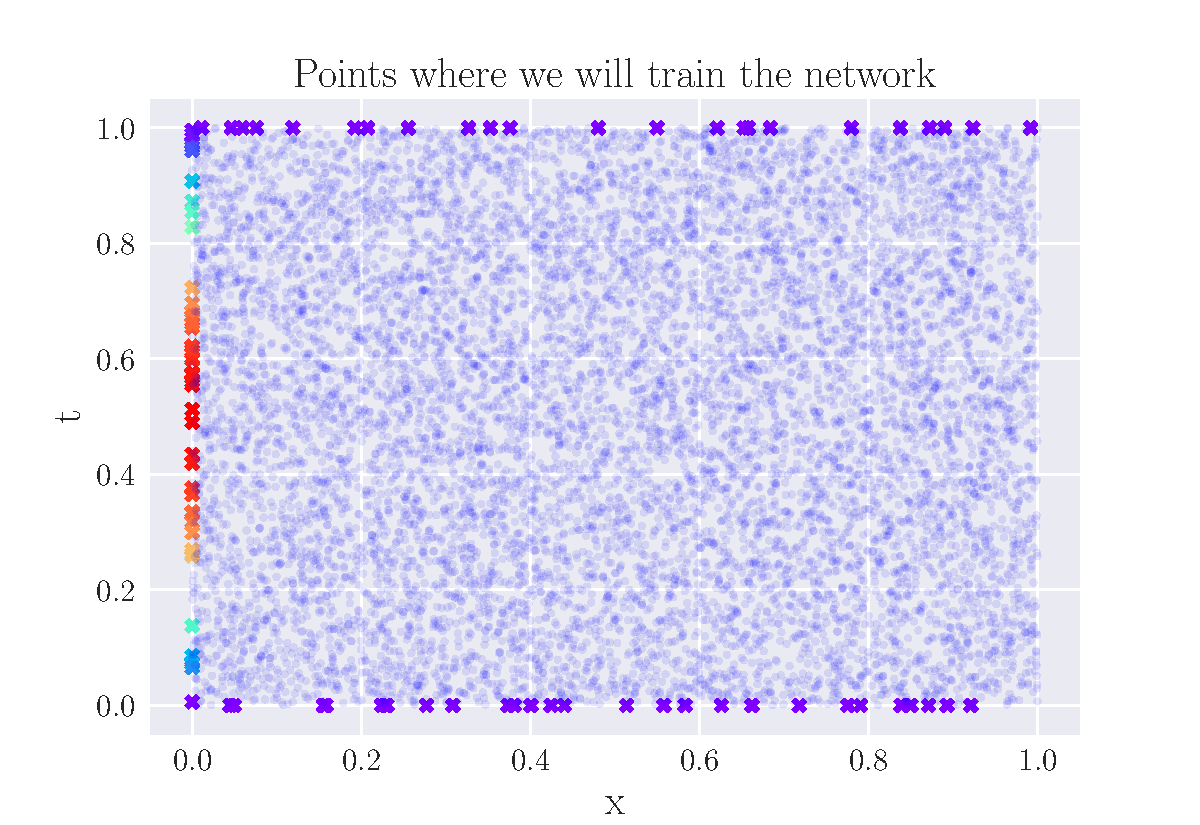
\includegraphics[width=\linewidth]{../output/plots/training_points.pdf}
	\caption{In this plot ...} \label{fig:NN_training_points}
\end{figure}

\begin{figure}[h]
	\minipage{0.49\textwidth}
	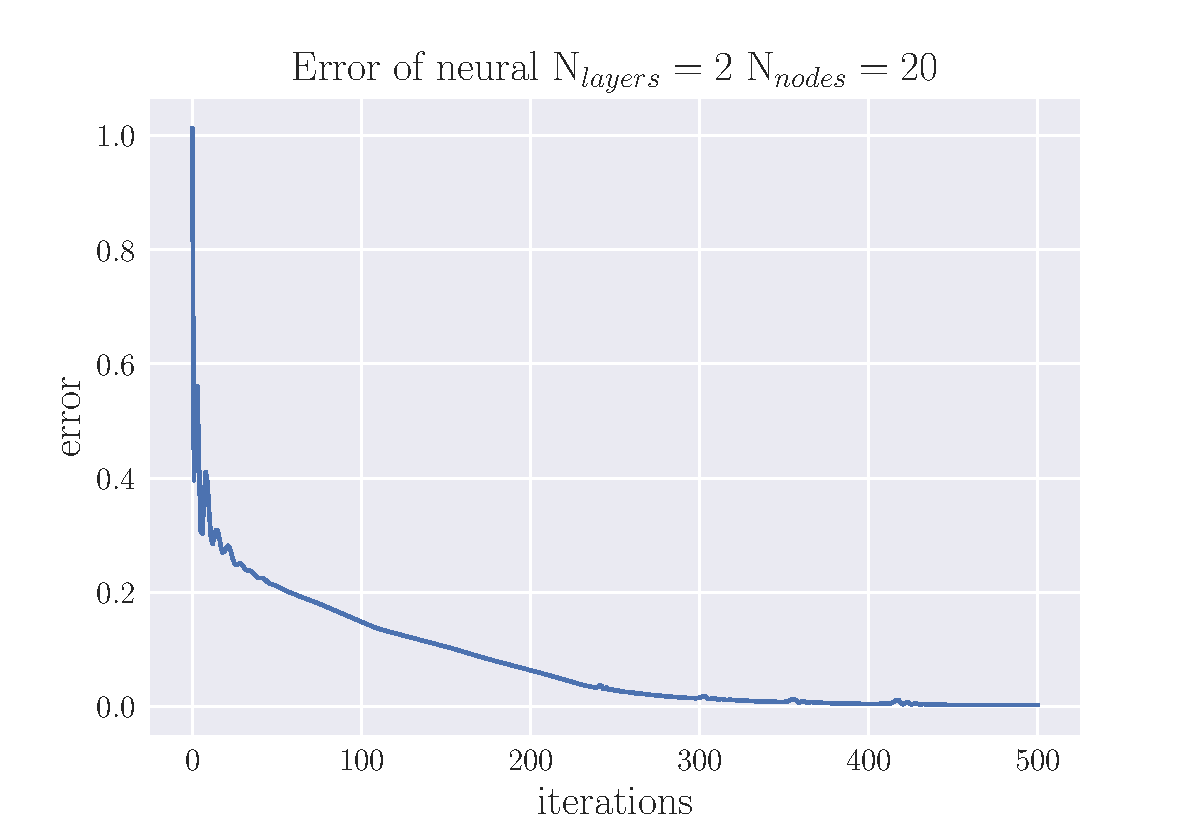
\includegraphics[width=\linewidth]{../output/plots/NN_diffusion_error_Nn20_Nh2.pdf}
	\endminipage\hfill
	\minipage{0.49\textwidth}
	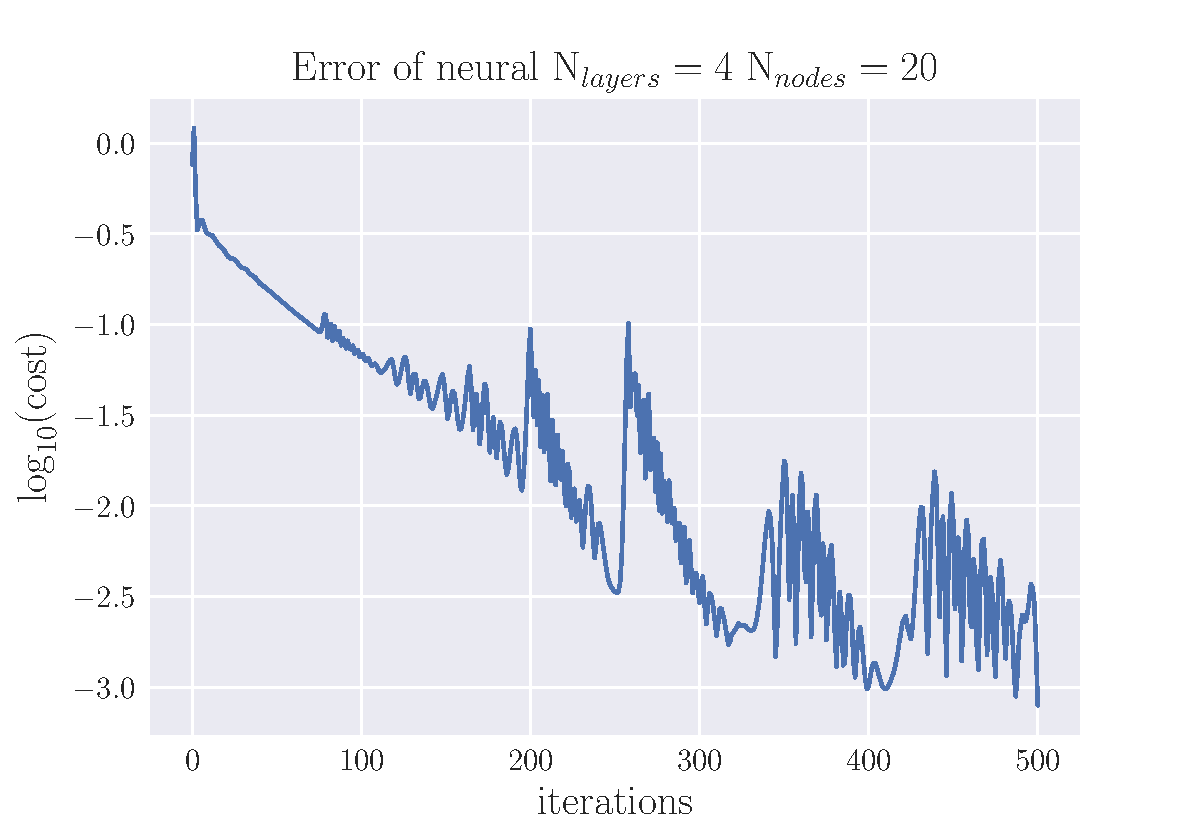
\includegraphics[width=\linewidth]{../output/plots/NN_diffusion_error_Nn20_Nh4.pdf}
	\endminipage\hfill
	\minipage{0.49\textwidth}
	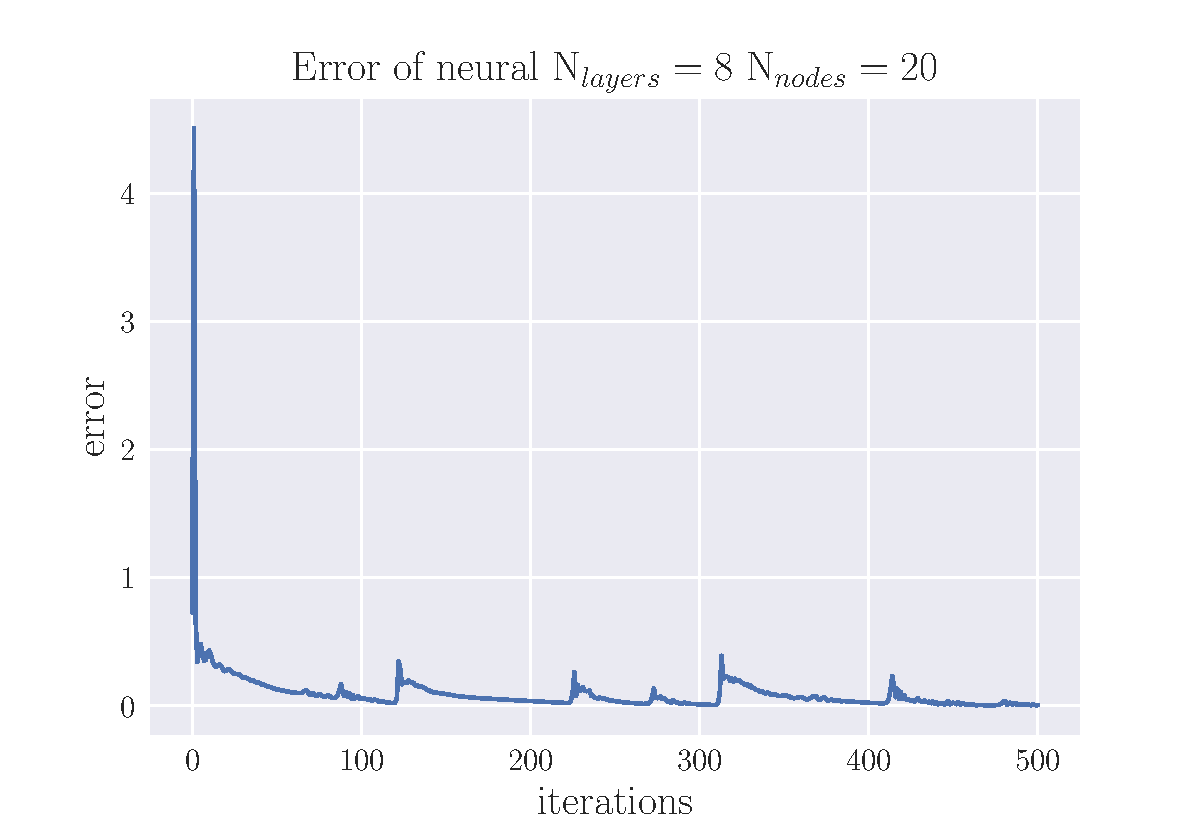
\includegraphics[width=\linewidth]{../output/plots/NN_diffusion_error_Nn20_Nh8.pdf}
	\endminipage\hfill
	\minipage{0.49\textwidth}
	\caption{Here ...} \label{fig:Error_NN_architecture}
	\endminipage
\end{figure}

\begin{figure}[h]
	\centering
	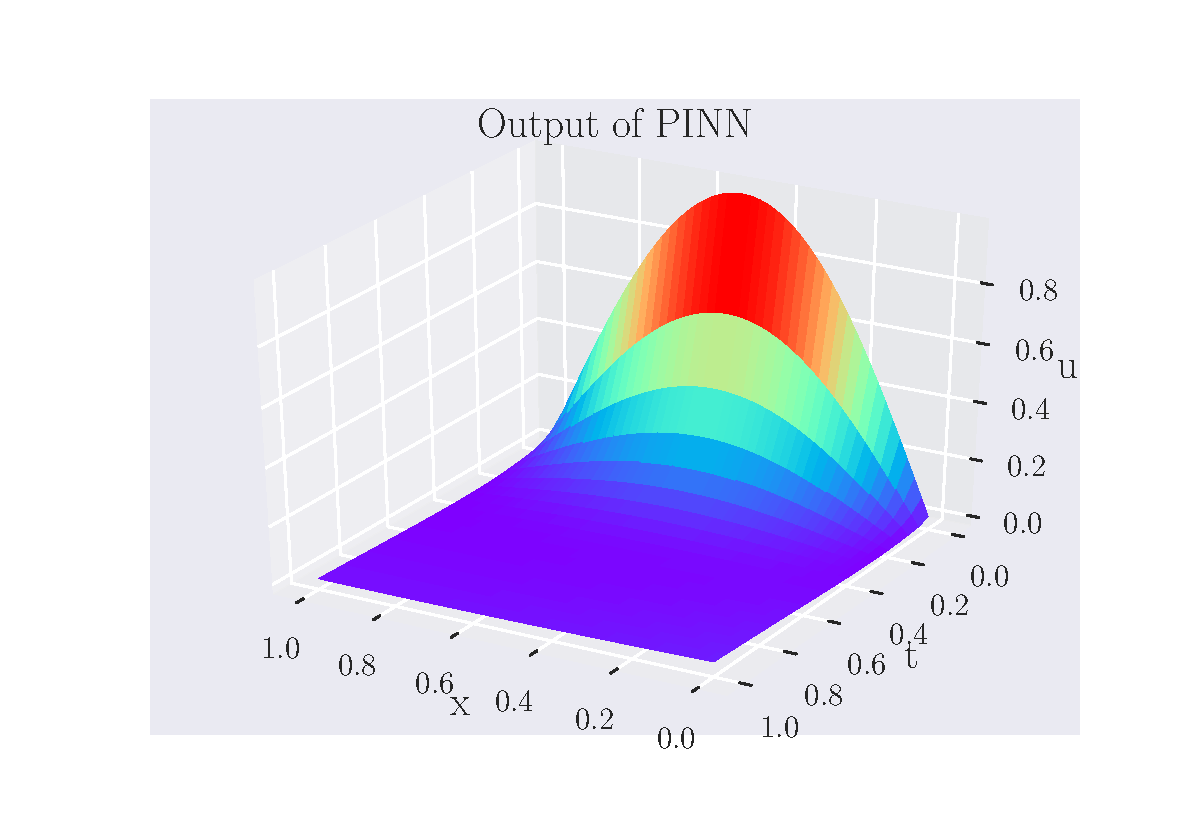
\includegraphics[width=\linewidth]{../output/plots/NN_diffusion_solution_Nn20_Nh4.pdf}
	\caption{In this plot ...} \label{fig:NN_architecture_solution}
\end{figure}

\begin{table}[h]
	\begin{tabular}{|l|l|}
		\hline
		Architecture & Error   \\ \hline
		$8\cross20$         & 0.00476 \\ \hline
		$4\cross20$         & 0.00079 \\ \hline
		$2\cross20$         & 0.00224 \\ \hline
	\end{tabular}
\end{table}


\clearpage
\subsection{Error of Forward Euler scheme}

To assess the accuracy of our implemented numerical scheme, we need to test the how well the produced solution fits the analytical solution. In this project we use the mean squared error to compare the approximated solutions with the analytical solution, both for forward euler and the neural network. Figure \ref{fig:FE_MSE} shows the MSE as function of time for the forward euler scheme. The time step is chosen to give a stability factor $\alpha=0.5$. The error increases significantly for early time steps, reaches a peak at around $t=0.1$ and quickly reduces thereafter. Already at $t=0.5$ the MSE is converging towards zero.

\begin{figure}[h]
	\centering
	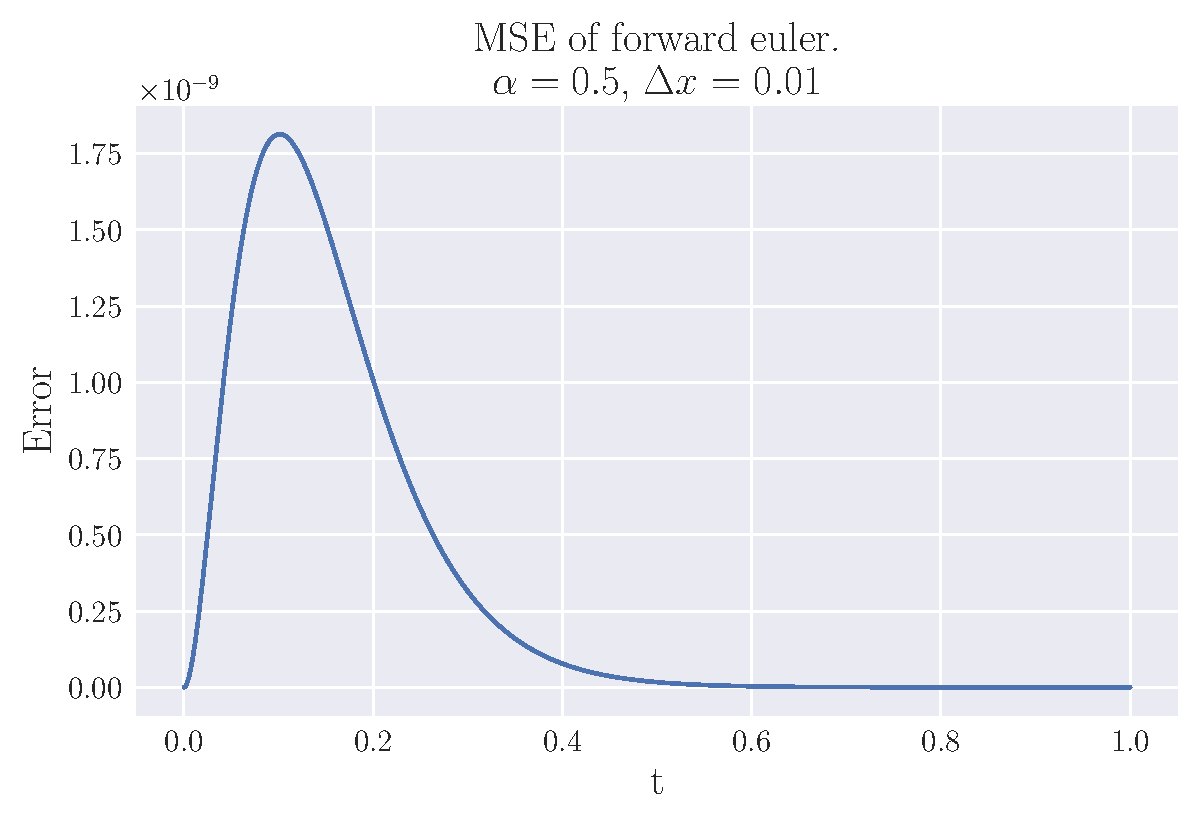
\includegraphics[scale=0.5]{../output/plots/MSE_FE_dx_001.pdf}
	\caption{Mean squared error of approximated solution by forward euler, using $\Delta x=0.01$ and time step $\Delta t$ dictated by the stability criterion \eqref{eq:stability}.}
	\label{fig:FE_MSE}
\end{figure}

Figure \ref{fig:NN_MSE} shows the MSE from the neural network with the architecture that provided best results. \textcolor{red}{Sigurd: Legg til MSE plottet her for det beste nettverket.}

Table \ref{tab:MSE_compare} compares the MSE obtained for forward euler and neural network at two selected time steps $t$ and two different spatial steps $\Delta x$. 


\begin{table}[h]
	\centering
	\begin{tabular}{l|ll|ll|}
		\cline{2-5}
		& \multicolumn{2}{l|}{\textbf{$\Delta x=0.1$}}           & \multicolumn{2}{l|}{\textbf{$\Delta x=0.01$}}           \\ \cline{2-5} 
		& \multicolumn{1}{l|}{\textbf{FE}}         & \textbf{NN} & \multicolumn{1}{l|}{\textbf{FE}}          & \textbf{NN} \\ \hline
		\multicolumn{1}{|l|}{\textbf{$t_1=0.1$}} & \multicolumn{1}{l|}{$1.72\cdot 10^{-5}$} &             & \multicolumn{1}{l|}{$1.81\cdot 10^{-9}$}  &             \\ \hline
		\multicolumn{1}{|l|}{\textbf{$t_2=0.5$}} & \multicolumn{1}{l|}{$1.50\cdot 10^{-7}$} &             & \multicolumn{1}{l|}{$1.69\cdot 10^{-11}$} &             \\ \hline
	\end{tabular}
\caption{MSE as function of spatial step $\Delta x$ for two different time levels, for forward euler scheme and neural network. Forward euler is abbreviated as FE and neural network as NN.}
\label{tab:MSE_compare}
\end{table}


\subsection{Error of Neural Network}

\textcolor{red}{Basert paa gammel figur. Sigurd: kanskje dette maa skirves om, avhengig av de endelige resultatene dine.}
Figure \ref{fig:error_NN_10000} shows the error of the neural network when approximating the solution $u_{\theta}$ to the actual solution $u$ as a function of training iterations. Initially, the error decreases considerably - it reduces by a factor of ten for just a couple of iterations, and the approximated solution improves significantly. Afterwards, the error decreases by a much slower rate with some minor fluctuations. Some time after 100 iterations the error is subject to a large jump, but quickly diminishes again. For later iterations the error slowly converges towards zero, possessing some irregular, minor fluctuations. 


\subsection{Comparison of error}


\subsection{Eigenvalue problem}


\begin{figure}[h!]
	\centering
	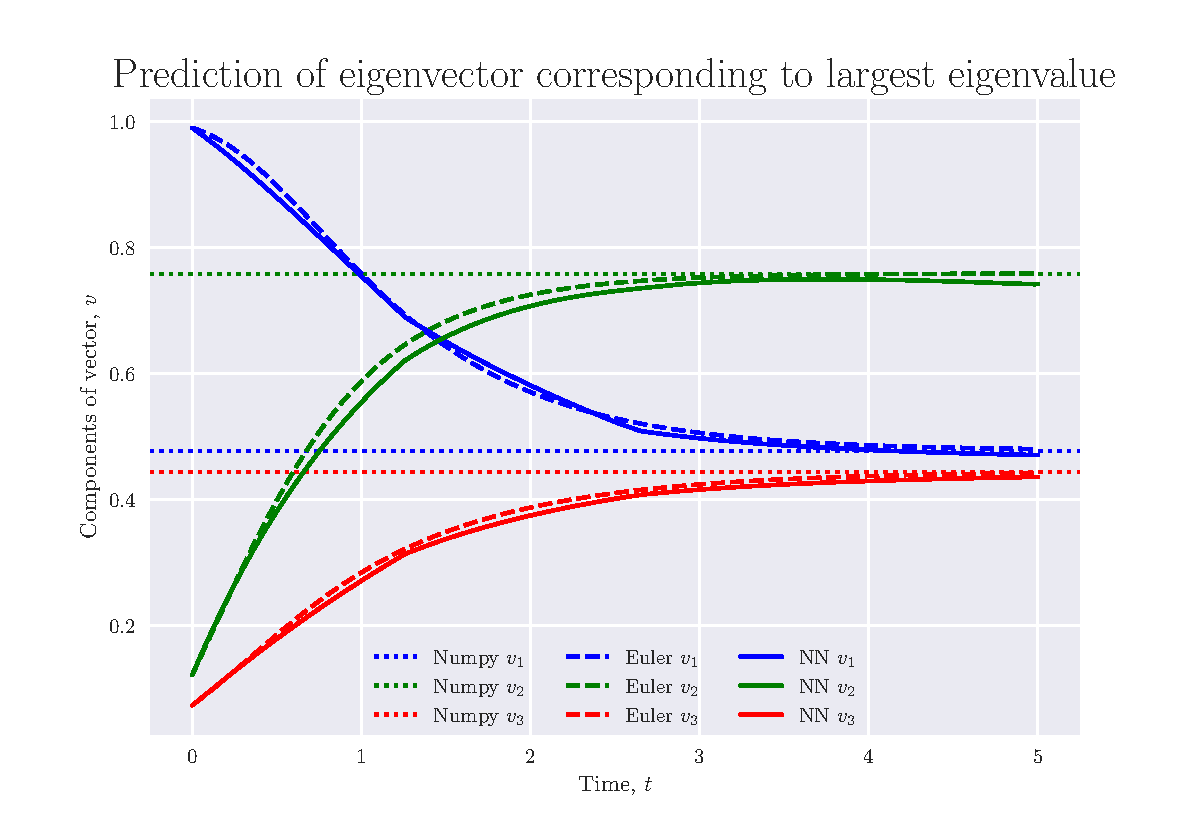
\includegraphics[scale=0.75]{../output/plots/eigvec_T5_N1000.pdf}
	\caption{Predictions by forward euler (FE) and neural network (NN) of the eigenvector corresponding to the largest eigenvalue of a real, symmetric $3\times 3$ matrix. The horizontal dotted lines are the components of the eigenvector as found by numerical diagonalization by \code{numpy.linalg.eig}.}
	\label{fig:eigvec_T5_N1000}
\end{figure}

\begin{figure}[h!]
	\centering
	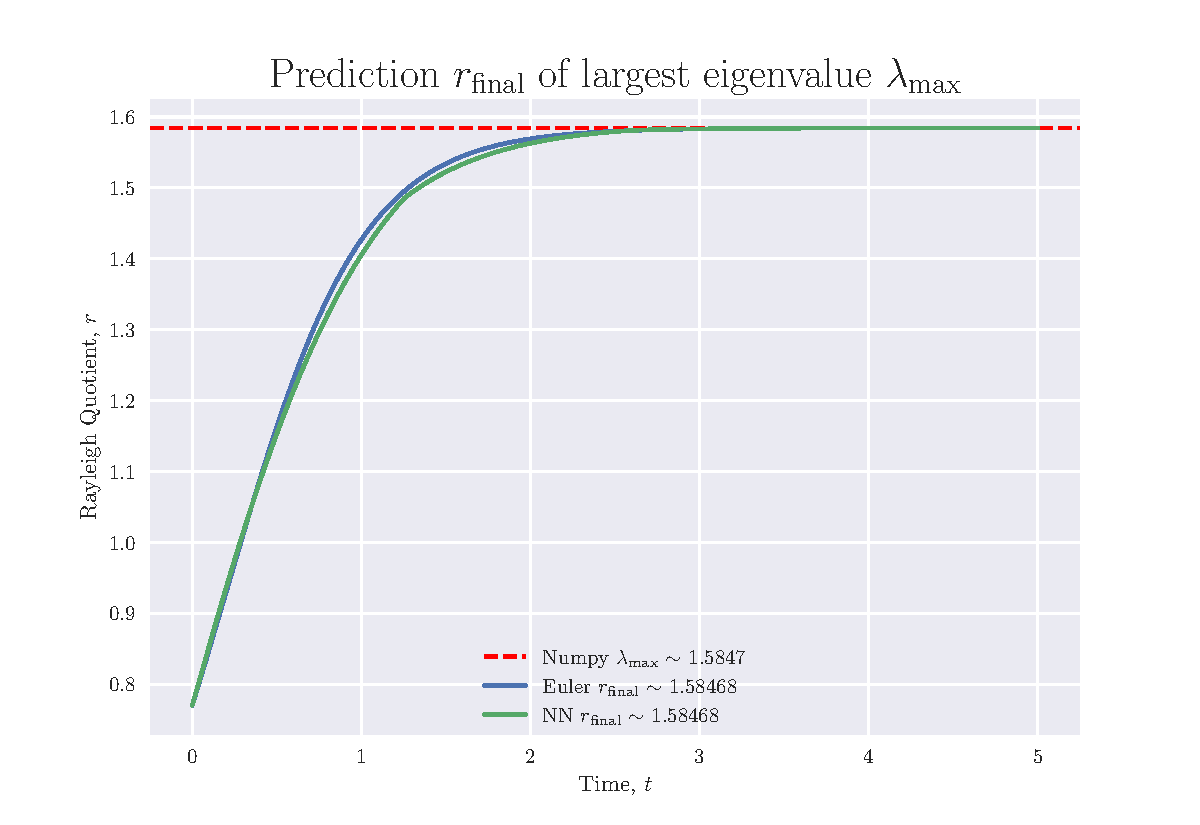
\includegraphics[scale=0.75]{../output/plots/eigval_T5_N1000.pdf}
	\caption{Rayleigh quotients of forward euler (FE) and neural network (NN) representing predictions of the largest eigenvalue of a real, symmetric $3\times 3$ matrix. The horizontal dotted line is the largest eigenvalue as found by numerical diagonalization by \code{numpy.linalg.eig}.}
	\label{fig:eigval_T5_N1000}
\end{figure}

Figure \ref{fig:eigvec_T5_N1000} shows predictions of the eigenvector corresponding to the largest eigenvalue of a symmetric $(3\times 3)$ matrix $A$ of randomly assigned values between 0 and 1. The simulation is run for a total time of $T=5$ with $N=1000$ estimations in time, providing a time step of $\Delta t = 0.005$. The prediction from both forward euler and neural network converges to the true eigenvector, as found by diagonalization with \code{numpy.linalg.eig}. The largest eigenvalue is shown in Figure \ref{fig:eigval_T5_N1000} together with the rayleigh quotients estimated by forward euler and the neural network.

\begin{figure}[h]
	
	\centering
	\begin{subfigure}{0.49\textwidth}
		\centering
		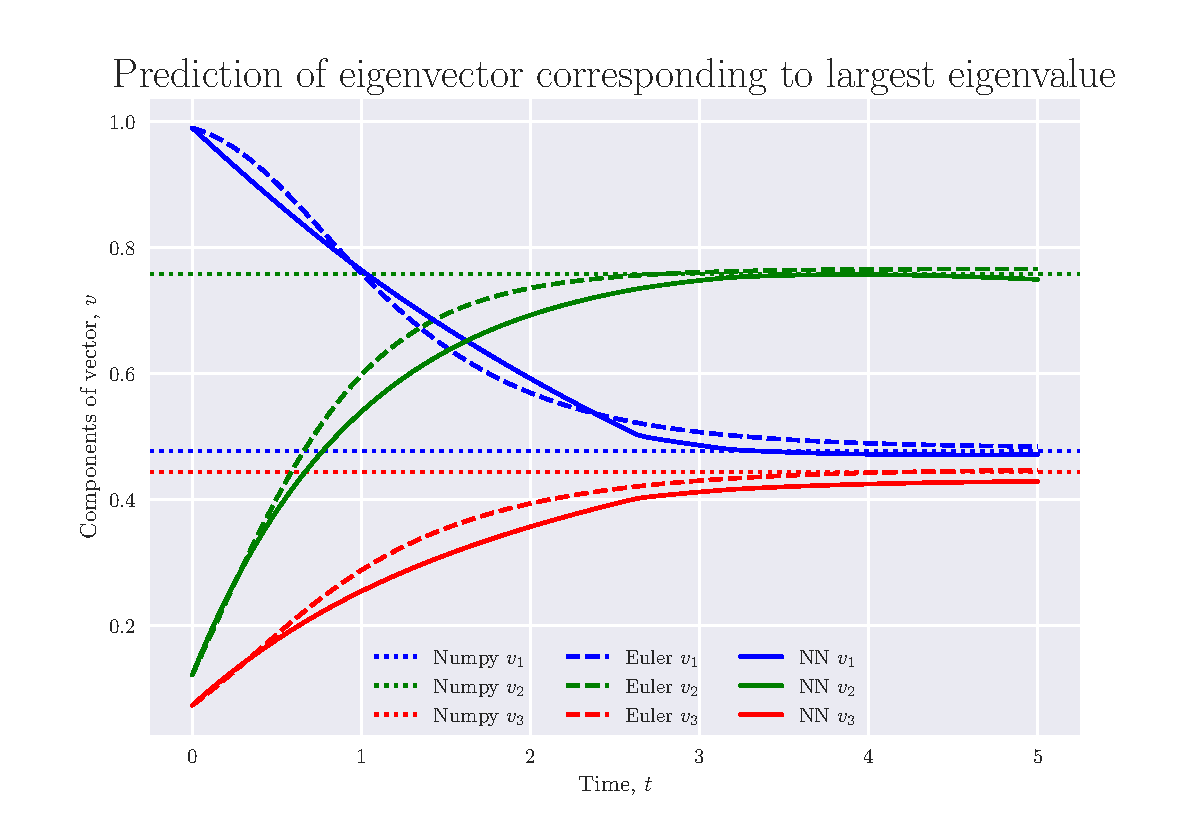
\includegraphics[width=\textwidth]{../output/plots/eigvec_T5_N100.pdf}
		\caption{Eigenvectors}
		\label{fig:eigvec_T5_N100}
	\end{subfigure}
	\hfill
	\begin{subfigure}{0.49\textwidth}
		\centering
		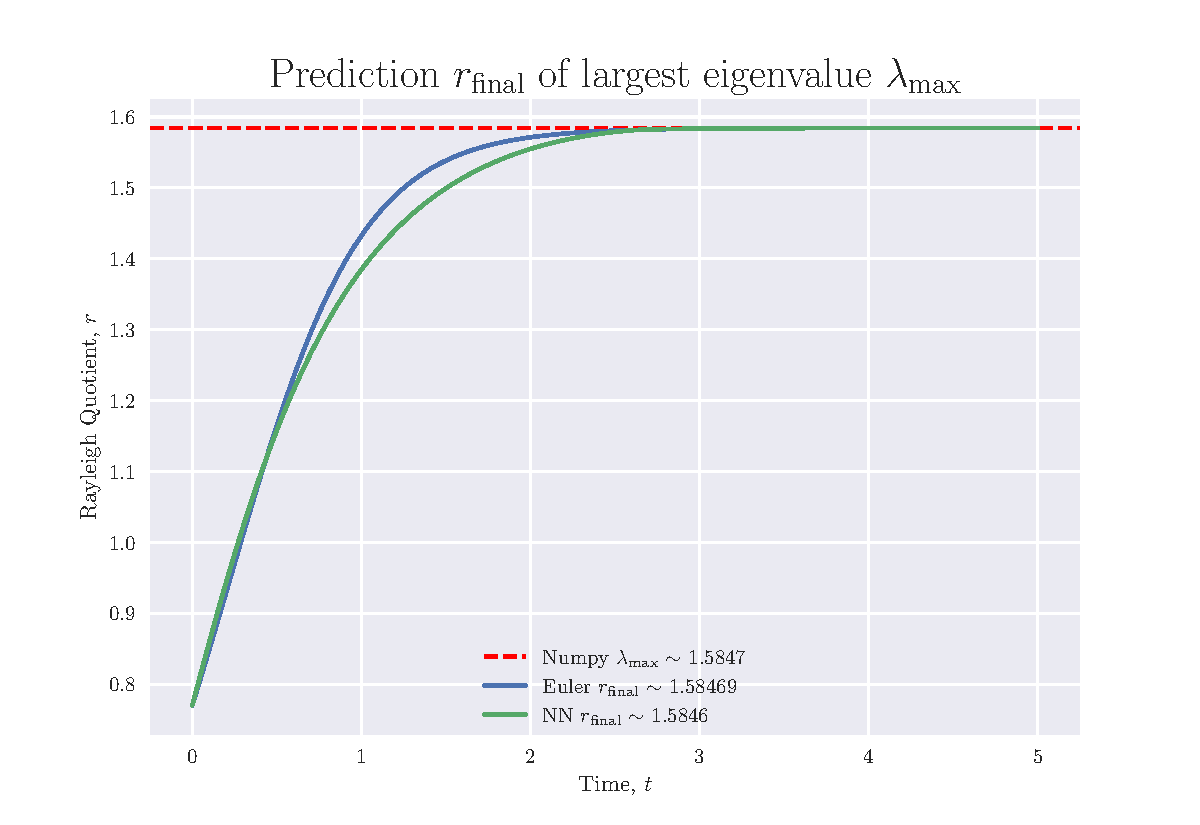
\includegraphics[width=\textwidth]{../output/plots/eigval_T5_N100.pdf}
		\caption{Rayleigh quotients}
		\label{fig:eigval_T5_N100}
	\end{subfigure}
	\caption{Predictions by forward euler (FE) and neural network (NN) of largest eigenvalue and corresponding eigenvector of a real, symmetric $3\times 3$ matrix, using a time step $\Delta t = 0.05$. The $x$ and $y$ axes are identical to those in figure \ref{fig:eigvec_T5_N1000} and \ref{fig:eigval_T5_N1000}}
	\label{fig:eig_T5_N100}
\end{figure}


\begin{figure}[h]
	
	\centering
	\begin{subfigure}{0.49\textwidth}
		\centering
		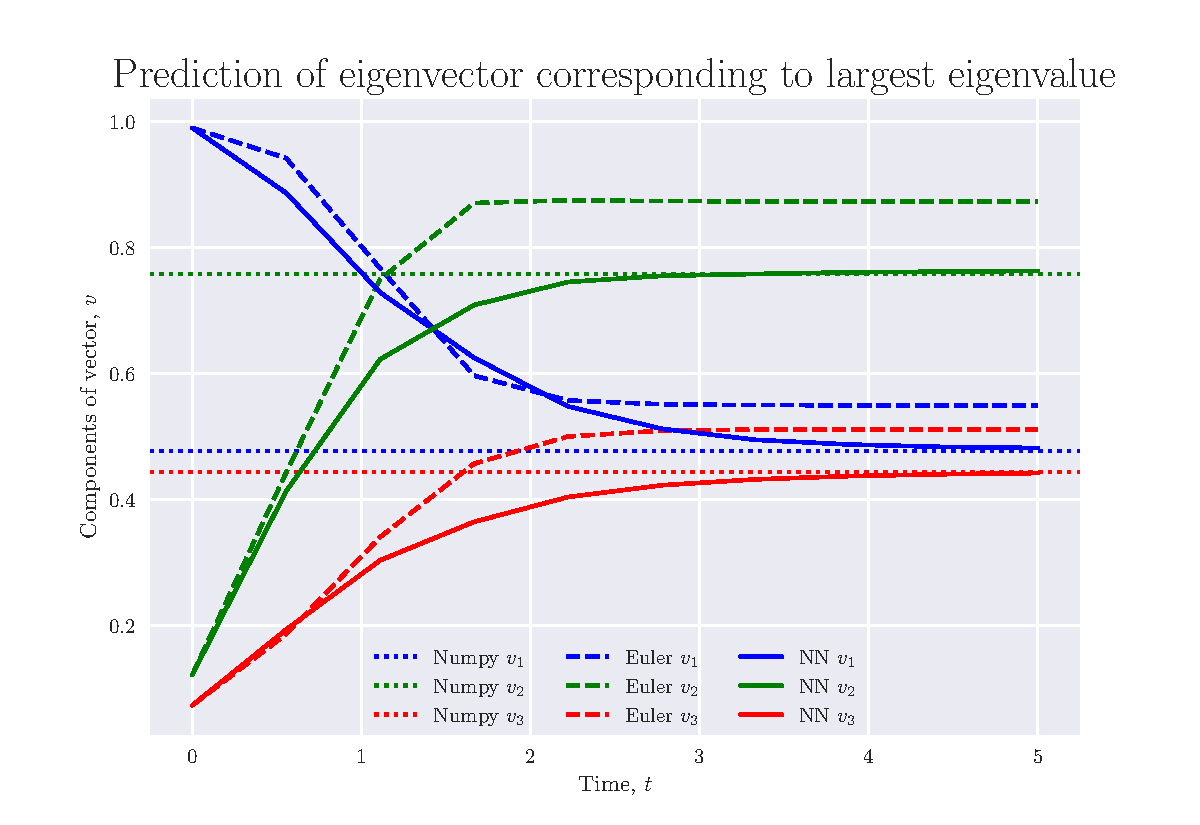
\includegraphics[width=\textwidth]{../output/plots/eigvec_T5_N10.pdf}
		\caption{Eigenvectors}
		\label{fig:eigvec_T5_N10}
	\end{subfigure}
	\hfill
	\begin{subfigure}{0.49\textwidth}
		\centering
		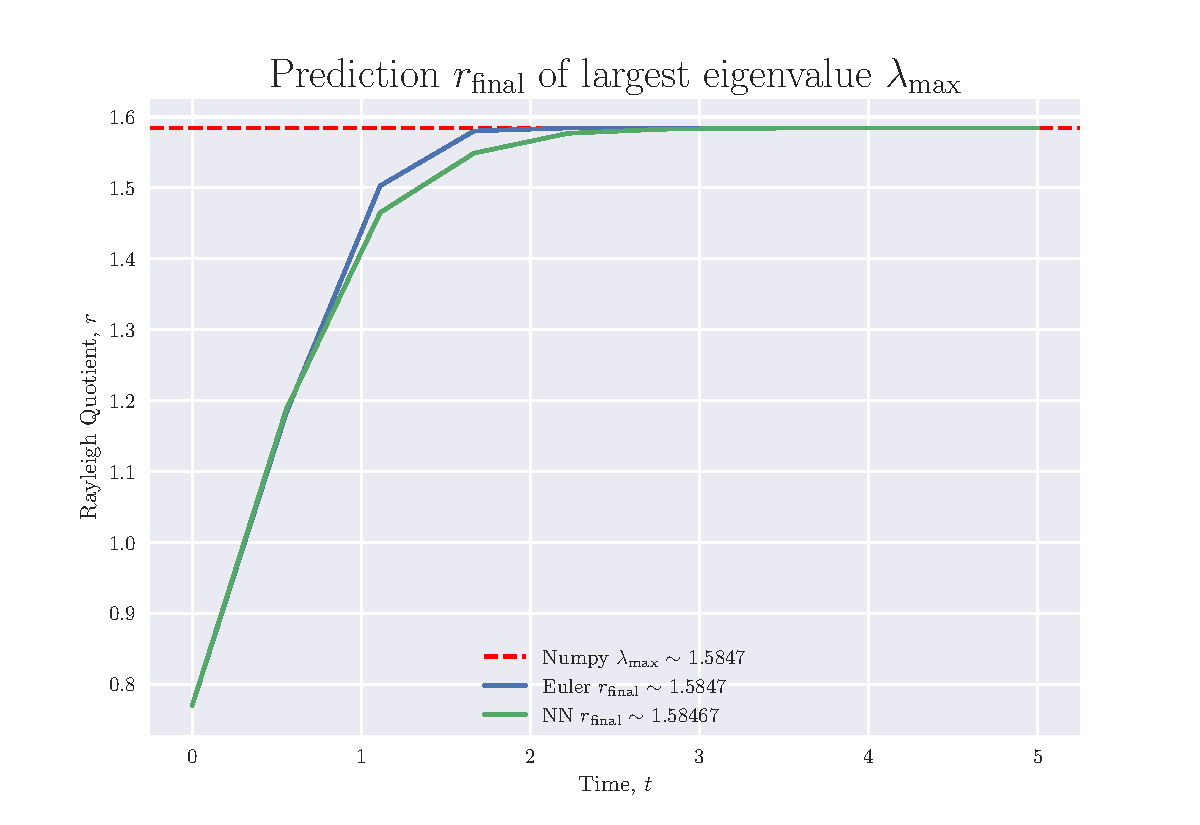
\includegraphics[width=\textwidth]{../output/plots/eigval_T5_N10.pdf}
		\caption{Rayleigh quotients}
		\label{fig:eigval_T5_N10}
	\end{subfigure}
	\caption{Predictions by forward euler (FE) and neural network (NN) of largest eigenvalue and corresponding eigenvector of a real, symmetric $3\times 3$ matrix, using a time step $\Delta t = 0.5$. The $x$ and $y$ axes are identical to those in figure \ref{fig:eigvec_T5_N1000} and \ref{fig:eigval_T5_N1000}}
	\label{fig:eig_T5_N10}
\end{figure}


Figure \ref{fig:eigvec_T5_N100} and \ref{fig:eigvec_T5_N10} shows predictions of the same eigenvector of the same matrix $A$ in Figure \ref{fig:eigvec_T5_N1000} but with a time step of $\Delta t = 0.05$ and $\Delta t = 0.5$, respectively. The largest eigenvalue and rayleigh quotients are shown in Figure \ref{fig:eigval_T5_N100} and \ref{fig:eigval_T5_N10}.
The graphs are less smooth due to larger timesteps and fewer estimates. 

\begin{figure}[h]
	
	\centering
	\begin{subfigure}{0.49\textwidth}
		\centering
		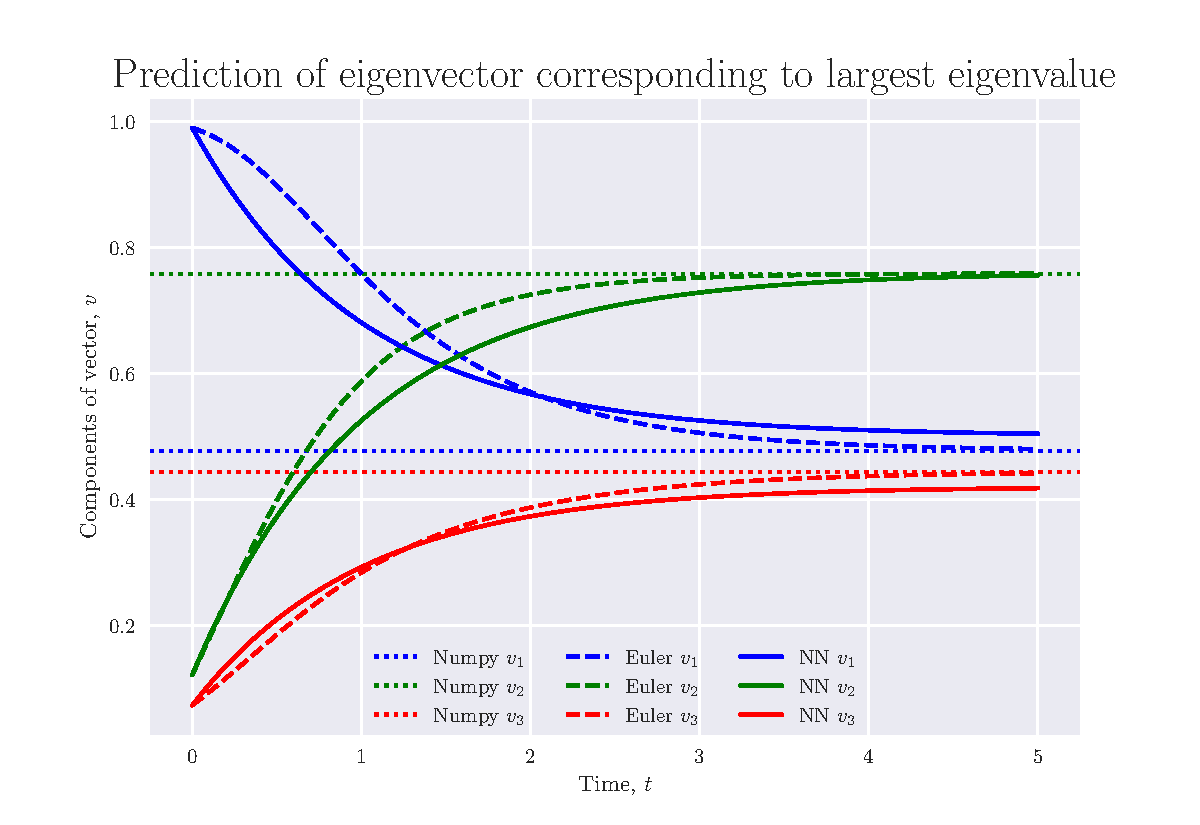
\includegraphics[width=\textwidth]{../output/plots/eigvec_T5_N1000_eta01.pdf}
		\caption{Eigenvectors}
		\label{fig:eigvec_T5_N1000_eta01}
	\end{subfigure}
	\hfill
	\begin{subfigure}{0.49\textwidth}
		\centering
		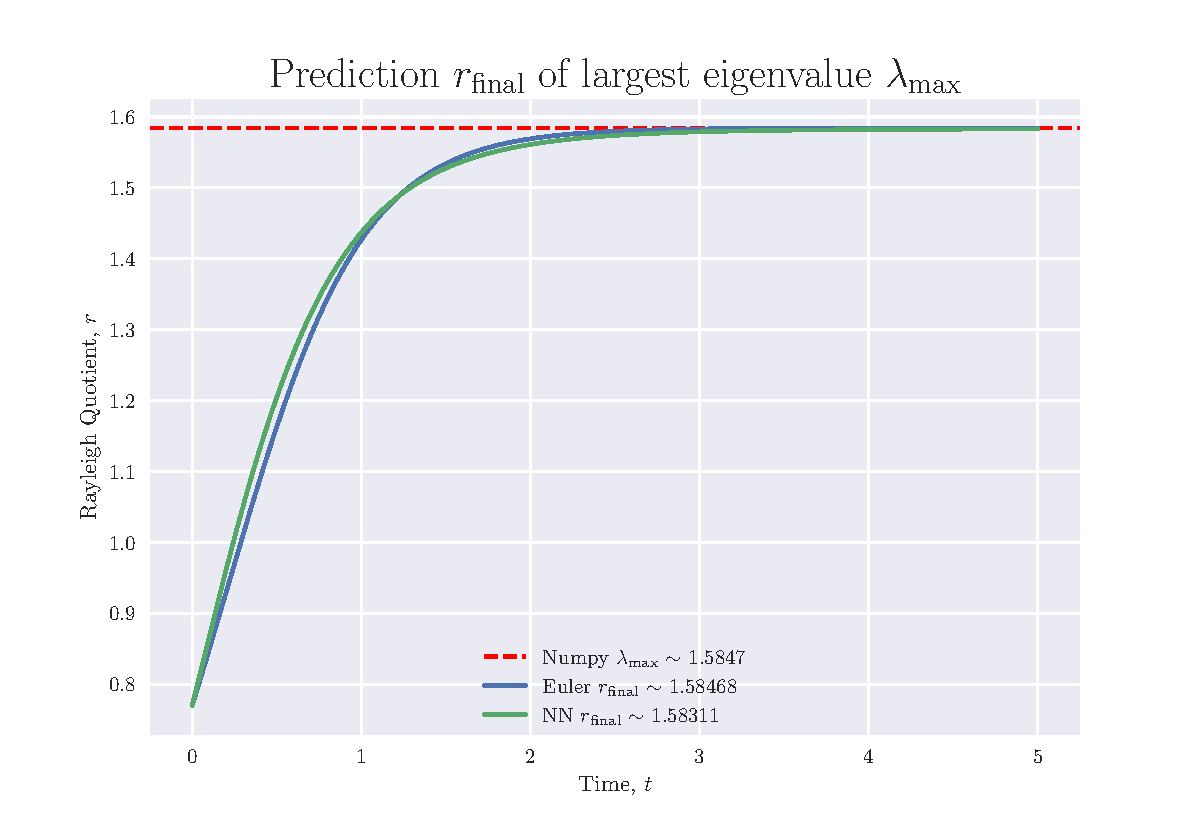
\includegraphics[width=\textwidth]{../output/plots/eigval_T5_N1000_eta01.pdf}
		\caption{Rayleigh quotients}
		\label{fig:eigval_T5_N1000_eta01}
	\end{subfigure}
	\caption{Predictions of largest eigenvalue and corresponding eigenvector by forward euler and neural network for a real, symmetric $3\times 3$ matrix, using a learning rate of $0.1$ and a time step $\Delta t = 0.005$. The $x$ and $y$ axes are identical to those in figure \ref{fig:eigvec_T5_N1000} and \ref{fig:eigval_T5_N1000}}
	\label{fig:eig_T5_N1000_eta01}
\end{figure}

\begin{figure}[h]
	
	\centering
	\begin{subfigure}{0.49\textwidth}
		\centering
		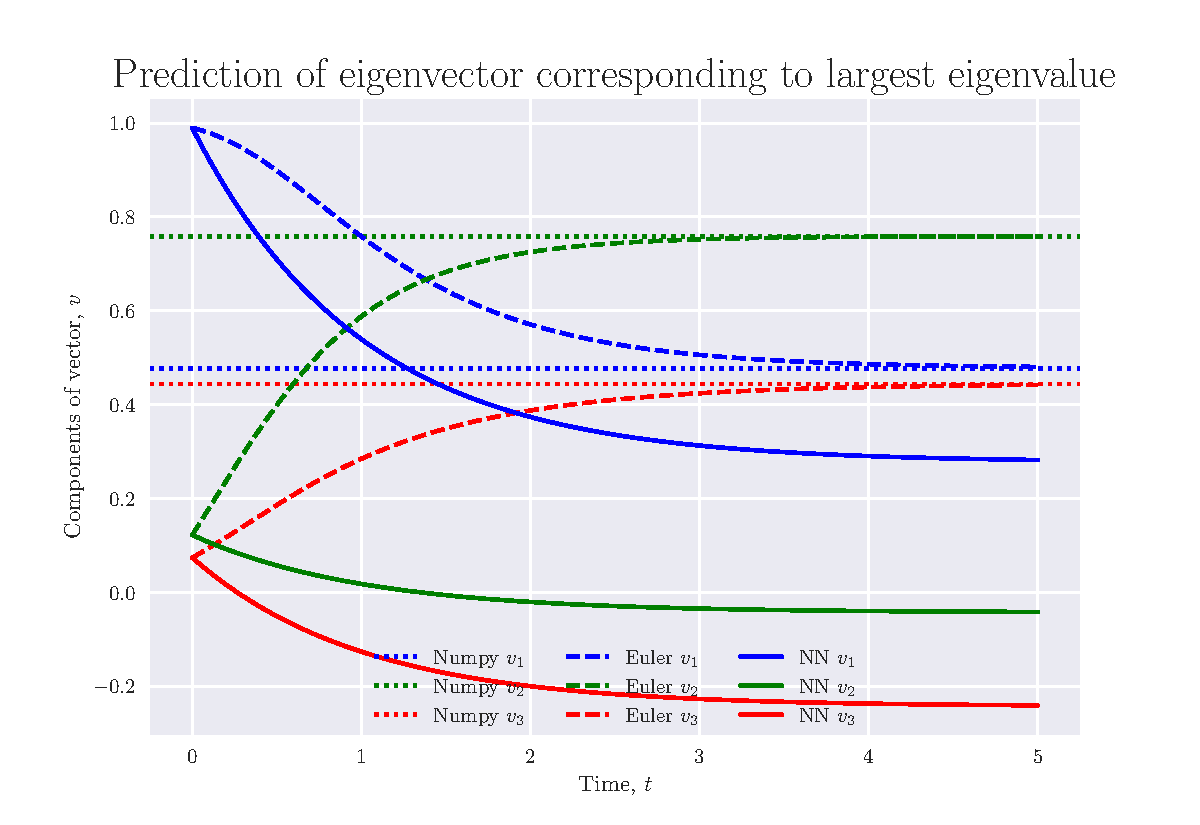
\includegraphics[width=\textwidth]{../output/plots/eigvec_T5_N1000_epochs50.pdf}
		\caption{Eigenvectors}
		\label{fig:eigvec_T5_N1000_epochs50}
	\end{subfigure}
	\hfill
	\begin{subfigure}{0.49\textwidth}
		\centering
		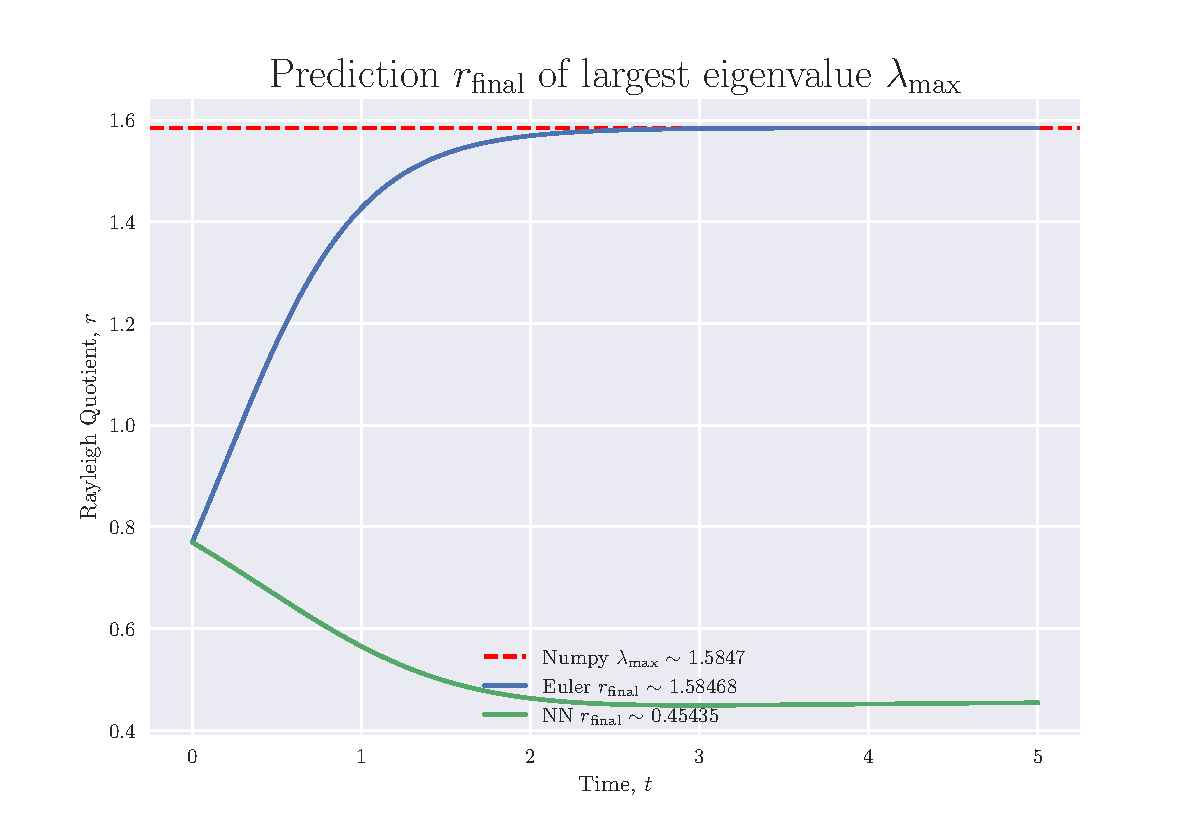
\includegraphics[width=\textwidth]{../output/plots/eigval_T5_N1000_epochs50.pdf}
		\caption{Rayleigh quotients}
		\label{fig:eigval_T5_N1000_epochs50}
	\end{subfigure}
	\caption{Predictions of largest eigenvalue and corresponding eigenvector by forward euler and neural network for a real, symmetric $3\times 3$ matrix, using a learning rate of $0.1$, $50$ epochs and a time step $\Delta t = 0.005$. Other than negative eigenvector components in the left panel, and lower Rayleigh quotient in the right panel, the $x$ and $y$ axes are identical to those in figure \ref{fig:eigvec_T5_N1000} and \ref{fig:eigval_T5_N1000}}
	\label{fig:eig_T5_N1000_epochs50}
\end{figure}


Adjusting hyperparameters of the neural network has also been investigated. Figure \ref{fig:eigvec_T5_N1000_eta01} shows the predicted eigenvector using a time step of $\Delta t = 0.005$ and a learning rate of $0.1$. The associated rayleigh quotients is shown in Figure \ref{fig:eigval_T5_N1000_eta01}. Predictions of the same eigenvector is shown in Figure \ref{fig:eigvec_T5_N1000_epochs50}, with the learning rate retained at $0.1$ but the number of epochs reduced from $2000$ to $50$. The associated rayleigh quotients are shown in Figure \ref{fig:eigval_T5_N1000_epochs50}.

\begin{figure}[h]
	
	\centering
	\begin{subfigure}{0.49\textwidth}
		\centering
		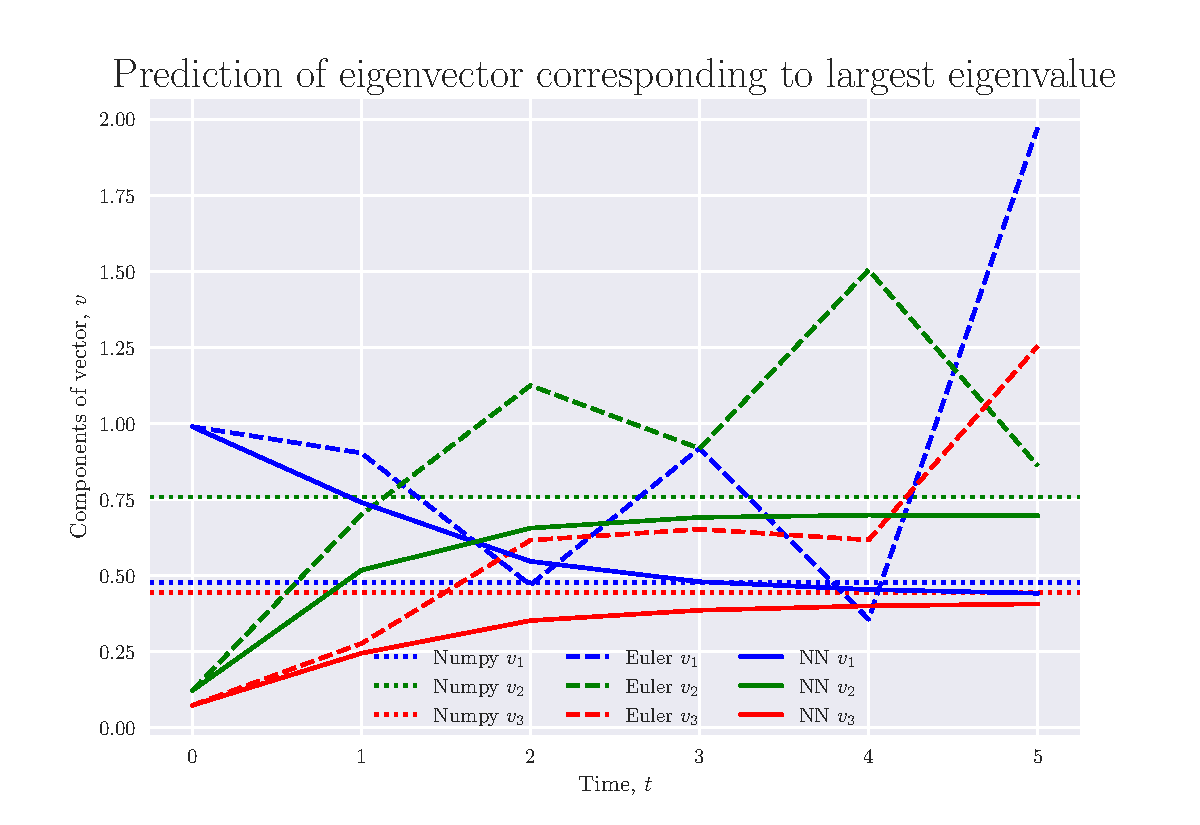
\includegraphics[width=\textwidth]{../output/plots/eigvec_T5_N6.pdf}
		\caption{Eigenvectors}
		\label{fig:eigvec_T5_N6}
	\end{subfigure}
	\hfill
	\begin{subfigure}{0.49\textwidth}
		\centering
		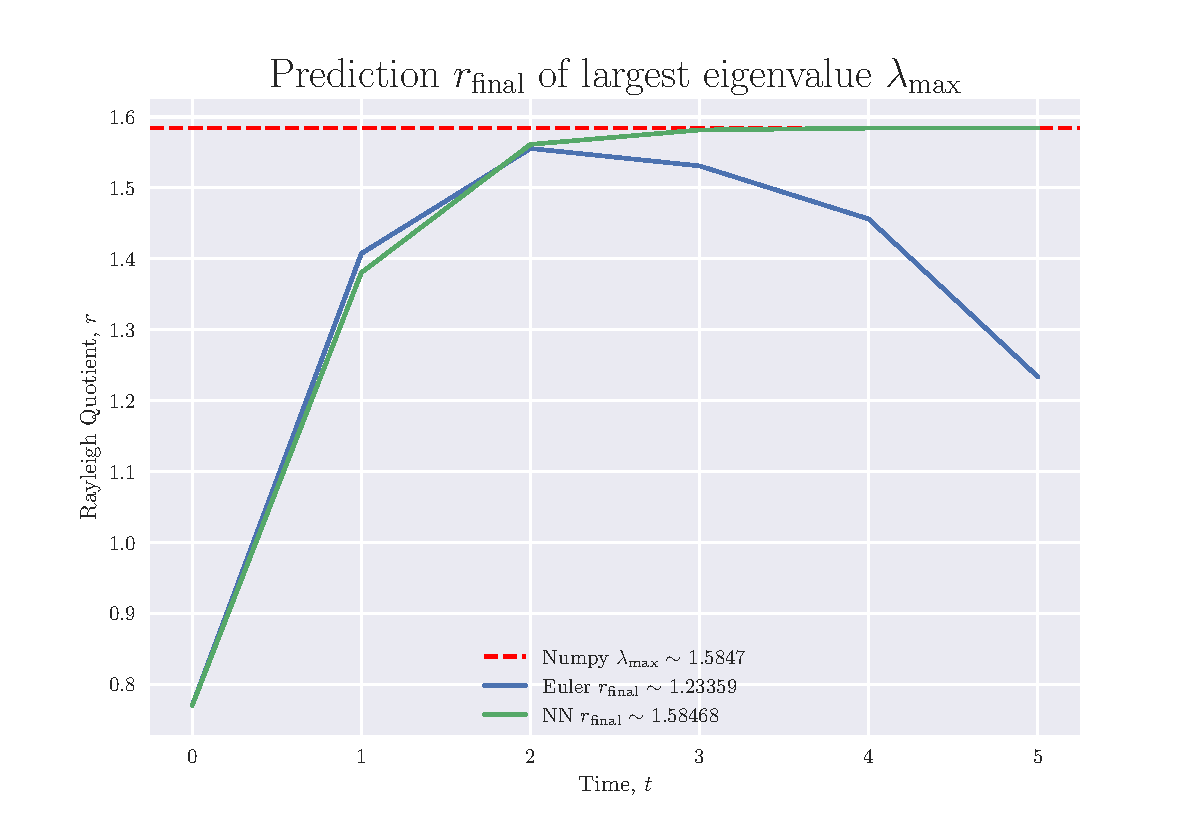
\includegraphics[width=\textwidth]{../output/plots/eigval_T5_N6.pdf}
		\caption{Rayleigh quotients}
		\label{fig:eigval_T5_N6}
	\end{subfigure}
	\caption{Predictions of largest eigenvalue and corresponding eigenvector by forward euler and neural network for a real, symmetric $3\times 3$ matrix. A time step of $\Delta t = 0.83$ is used. Other than increased eigenvector component values for forward Euler on the left panel, the $x$ and $y$ axes are identical to those in figure \ref{fig:eigvec_T5_N1000} and \ref{fig:eigval_T5_N1000}}
	\label{fig:eig_T5_N6}
\end{figure}

Results of a further increase in the time step is shown in Figure \ref{fig:eig_T5_N6}, using $\Delta t= 0.83$ corresponding to $N=6$ estimations, where the left panel shows the eigenvector components and the right panel shows the associated Rayleigh quotients. 

 
\clearpage
\section{Discussion}

\subsection{Solving the diffusion equation with Forward Euler}
Figure \ref{fig:FE_MSE} verifies that simulating the forward euler scheme of the diffusion equation with spatial step $\Delta x = 0.01$ yields an excellent correspondance between the numerical and analytical solution. The maximum error is obtained at an early time step, around $\Delta t = 0.1$. For time levels beyond this, the MSE decreases exponentially and eventually converges towards zero. Notice that the error is exactly zero initially, because the numerical scheme has enforced the solution at the initial time step to satisfy the initial condition from the analytical solution. The maximum error is on the order of $10^{-9}$, yielding an excellent fit to the exact solution. One would not be able to distinguish the numerical solution from the exact solution if they were plotted together.

\par The shape of the plot is in good correspondance with what was initially expected, as elaborated on in Methods. The large initial increase of the MSE is a result of the curved initial solution. The spatial gradients are significant and the approximation with finite differences becomes less accurate.
In the beginning of the diffusion process, for low $t$, the solution changes rather quickly. The forward euler scheme is first order accurate in time, $O(\Delta t)$, and second order accurate in space, $O(\Delta x^2)$, implying that the numerical solution is more sensitive to the temporal evolution than the spatial evolution. Hence, the forward euler scheme will produce larger errors for the initial time levels due to the rapid change in solution \cite{Linge2017}.
\par After time $t=0.1$ the MSE decreases. This can be explained by the discretization parameters $\Delta t$ and $\Delta x$. The magnitude of the gradients are diminished because the solution becomes more linear and less curved. As a result, the solution changes more slowly, allowing the finite difference scheme to approximate the changes more accurately both spatially and temporally. Eventually, the exact solution is approximately constant at zero. In this case, the gradients of the solution are indiscernible and the numerical scheme is able to approximate the solution with machine precision. Figure \ref{fig:FE_MSE} illustrates this by the MSE converging towards zero sufficiently deep into the diffusion process.

\subsection{Solving the diffusion equation with a neural network}

\par \textcolor{red}{Et forsøk paa aa forklare fluktuasjonene i MSE for NN:} The reason that the error flucuates instead of decreasing monotonically is that we use the Adam optimizer [\textcolor{red}{https://arxiv.org/abs/1412.6980}]. This is a type of stochastic optimization method, providing more favorable features than traditional stochastic methods. The stochasticity allows the neural network to explore more of the convex parameter space by trying out new, potentially worse solutions. The hope is that, after escaping the local optima, that we find an even better solution at some later stage. The apparent jump in Figure \ref{fig:error_NN_10000} is an example of escaping a local optima at the expense of further exploration. In this case, it does not seem like the new solutions lead to better performance than the previous optima. It eventually converges to zero, which is something the solutions prior to the jump did as well. 

\subsection*{Using Forward Euler and Neural Network to find eigenvalues}
Forward euler and neural networks are two different numerical methods capable of finding the eigenvalues of a real, symmetric matrix $A$ by solving the ODE in equation \eqref{eq:diff_eig}. The two algorithms for solving differential equations are quite different, and will therefore yield different predictions of the largest eigenvalue. The result of forward euler is sensitive to the time step $\Delta t$. Thus, it is of interest to compare the accuracy of prediction of the two methods when the time step is altered. 

% FE: N=1000, N=100, N=10
Comparing Figure \ref{fig:eigvec_T5_N1000}, Figure \ref{fig:eigvec_T5_N100} and Figure \ref{fig:eigvec_T5_N10} for time steps $\Delta t = 0.005$, $\Delta t = 0.05$ and $\Delta t = 0.5$, respectively, we observe that the accuracy of forward euler consistently decreases for larger time steps. The result for $\Delta t=0.5$ is particularly biased with all components of the predicted eigenvector consistently missing their respective targets. The corresponding rayleigh quotients, shown in Figure \ref{fig:eigval_T5_N1000}, Figure \ref{fig:eigval_T5_N100} and Figure \ref{fig:eigval_T5_N10}, converge precisely to the largest eigenvalue calculated by \code{numpy.linalg.eig}. Thus, despite the lower accuracy - particularly for forward euler - both methods succeed in returning the largest eigenvalue with four decimal precision.

It may appear surprising that the significant bias of the estimated eigenvector for forward euler for $\Delta t =0.5$ is not replicated in the associated rayleigh quotient, which converges precisely to the largest eigenvalue. To explain this, observe that the \textit{relation} between the components of the estimated eigenvector seems to replicate that of the true eigenvector, only shifted towards higher values. If $v$ is the eigenvector of matrix $A$, the associated eigenvalue is given by
\[ \lambda = \frac{v^T A v}{v^T v} \]
Then, if $s$ a constant representing the shift, the rayleigh quotient becomes

\begin{align*}
	r &= \frac{(sv)^T A (sv)}{(sv)^T (sv)} = \frac{s^2 v^T A v}{s^2 v^T v} \\
	&= \frac{v^T A v}{v^T v}
\end{align*}

This implies that the associated eigenvalue is unaffected by scaling the components of an eigenvector by a constant amount. Geometrically, it means that the eigenvector is extended or shrunk, but the spanned eigenspace is the same, hence the same eigenvalue. \textcolor{red}{Gir dette mening, Vikenes, Sigurd? Vikenes: Ja.} Figure \ref{fig:eig_T5_N1000_eta01} is an exception, though. For this particular simulation, the relation between the first and third predicted eigenvectors are different from the relation of the true eigenvectors, whereas the rayleigh quotient converges to the largest eigenvalue. This does not comply with the argument above, and we find it difficult to interpret this particular result. It should incentivate for further analysis.

% NN: N=1000, N=100, N=10
The neural network on the other hand, apparently looks unaffected by the increase in time step. In fact, it seems like the neural network has a more accurate convergence for $\Delta t = 0.5$ than $\Delta t = 0.05$ and $\Delta t = 0.005$. Still, this does not imply that the accuracy increases with larger time step in general, but it substantiates the fact that the convergence property of a neural network is more sensitive to other features than the time step. 

% NN: Dependence on other params than time step
In project 2 we studied some of the most sensitive parameters for a neural network to provide accurate predictions, including the learning rate, number of epochs and loss function. The dependence on the learning rate is illustrated by comparing Figure \ref{fig:eigvec_T5_N1000} with \ref{fig:eigvec_T5_N1000_eta01}. Increasing the learning rate from 0.005 to 0.1 has consequences for the result. The neural network now predicts an eigenvector whose components notably deviate from that of the true eigenvector. From Figure \ref{fig:eigval_T5_N1000_eta01} the rayleigh quotients corresponds quite well with the largest eigenvalue, just slightly less accurate. Additionally, if the number of epochs is reduced to 50, the consequences are even more severe, as shown in Figure \ref{fig:eigvec_T5_N1000_epochs50}. Now the predicted components completely misses the true components of the eigenvector. Figure \ref{fig:eigval_T5_N1000_epochs50} shows that the rayleigh quotients of the neural network apparently converges to a different value than the largest eigenvalue. Because forward euler only depends on $\Delta t$, it is unaffected by a change in the learning rate and number of epochs. Conclusively, the results indicate that a learning rate of $0.1$ and $50$ number of epochs is not a good architecture of a neural network for solving equation \eqref{eq:diff_eig}.


% FE & NN: N=1000, N=100, N=10
Figure \ref{fig:eigvec_T5_N6} shows that the eigenvector components do not converge but rather oscillate in an inconsistent pattern when we use Forward Euler with a time step $\Delta t =0.83$. There is a strong indication of diverging values for the eigenvector components, which would be more apparent if we either increased the duration of the simulation, or decreased the time step even further. 

 The corresponding rayleigh quotients, shown in Figure \ref{fig:eigval_T5_N6}, verify that forward euler is not able to converge to the true solution of equation \eqref{eq:diff_eig} as $\Delta t$ is too large. All simulations with $\Delta t \leq 0.5$ have given a relative error less than $1\%$ between the final rayleigh quotient and the largest eigenvalue using forward euler. In comparison, the relative error for $\Delta t = 0.83$ is $22.1\%$.

Taking all simulations into account, the neural network has excellent accuracy for $\Delta t < 1$. This indicates weak dependency on the time step, but this is completely deafed by the sensitivity to other hyperparameters such as learning rate and number of epochs.



\subsection{Potential for solving general differential equations}
The forward euler method and neural networks are two quite different methods for solving differential equations. The former relies on discretization of the derivative to arrive at an explicit recursive set of equations to solve for each time step. The latter uses the residual error from the approximation as a basis for backpropagation to update weights and biases to improve the approximation to the actual solution. Figure \ref{fig:error_NN_40000} visualizes how bad the approximated solution of the initial run of the neural network is. Just after a few iterations though, the error decreases tremendously and goes below 0.083 (which is the total error obtained from forward euler) after around 100 iterations. After this, the total error fluctuates mildly but eventually converges towards zero.
 
\par The forward euler method clearly has an advantage in its simple recursive formula and fast computation time. The proposed solution is calculated within a few milliseconds, with a total error of only 0.083. On the other hand, it is limited by a stability requirement in order to produce realistic results. This effectively puts a restriction on applicable mesh resolutions.

\par A notable drawback of the neural network is the demanding training process. To compute an approximated solution of \eqref{eq:diffusion_equation_1D} requires calculating gradients and accumulating chained derivatives backwards through the hidden layers. This is a significantly larger computational effort than calculating the simple recursive formula of the forward euler scheme. As a result, the neural network suffers from a large computational runtime. Still, if training sufficiently long, the neural network will produce a better solution than forward euler and eventually yield a near perfect approximation to the exact solution. 

\par The forward euler scheme has proven to obtain good accuracy on the numerical solution. However, forward euler has an inherent disadvantage in that it is conditionally unstable with stability criteria given by \eqref{eq:stability}. In general it means that the forward euler scheme is not a stable method for solving differential equations as it requires that we carefully assign the mesh discretization steps. Neural networks are not limited to any kind of discretization. Neural networks benefit from good convergence properties. That is, given enough time to train it is able to approximate the actual solution of a differential equation with an error of approximately zero. Moreover, the neural network model \eqref{eq:NN_model} has the additional flexibility in that the function $f$ can be tweaked to give a better initial guess of the solution. 
\par Overall, the method of choice for solving differential equations is a tradeoff between the accuracy of the approximated solution and the computational runtime. Forward euler is definitely the desired method if we want a quick representation of the solution. If the importance is how precise the representation is, a neural network is a better choice.

\textcolor{red}{Det meste av diskusjonen over kan beholdes da det gjelder generelt, men de faktiske tallene nevnt maa oppdateres med resultatene fra MSE.}


\subsection{Eigenvalue problems}
The potential of solving differential equations spans a large domain of mathematical problems. Particularly, the model \eqref{eq:diff_eig} can be represented by a neural network or a forward euler scheme to approximate the eigenvalues of a real, symmetric matrix. Our experiments have shown that the neural network has no trouble finding an accurate approximation to the largest eigenvalue and the corresponding eigenvector given a suitable trial solution and network architecture. The parameter space of a neural network is large, and optimizing a solution requires an infeasible search over all parameters. Training for more epochs gives a more accurate prediction, but comes at the expense of a longer runtime, in which case forward euler can produce equally accurate results for a much shorter runtime. Nonetheless, the optionality to tune the various parameters of a neural network makes it a flexible method for finding approximate solutions.

The forward euler scheme gives a more accurate prediction then the neural network, in addition to converging faster, as long as the time step is sufficiently low. In this case, forward euler is the prevailing method for finding the largest eigenvalue of a real, symmetric matrix. However, the method has an inherent disadvantage in terms of stability. Our experiments indicate that forward euler diverges for $\Delta t \ge 1$. This marks a transition where the results of forward euler are deceptive and the neural network is the method of choice.

Most of the differential equations frequently applied in natural science, such as the diffusion equation, are simple enough for finite difference schemes to handle efficiently and accurately. However, for more intricate differential equations finite differencing may not give accurate approximations of gradients. Refining the mesh is a solution, but discretization parameters eventually become low enough to yield stability issues, particularly for forward euler. A refinement of the mesh is also necessary when simulating for very long time periods. For these particular cases, it seems like neural network is the prominent method and a great alternative to conventional numerical schemes. Hence, the method of choice is problem specific. 

\textcolor{red}{Vikenes: Burde kommentere at NN vil være bedre/raskere for mer komplekse modeller, og at NN er best dersom man skal simulere over lange perioder.}



\section{Conclusion}
Hei, i prosjekt 3 har vi valgt oppgaven om diff-likninger.
Vi hadde nettopp fullført oppgave d) ang. egenverdi

\section{Appendix}

\section*{Appendix}

\subsection*{Analytical solution of the diffusion equation}
By using the concept of separation of variables, the solution can be expressed as
\[ u(x,t) = X(x)T(t) \]
The solution is separated into a function $X$ only depending on the independent variable $x$, and a function $T$ only depending on the independent variable $t$. Equation \eqref{eq:diffusion_equation_1D} can then be rewritten as

\begin{align*}
	\frac{\partial^2 X(x)T(t)}{\partial x^2} &= \frac{\partial X(x)T(t)}{\partial t} \\
	T(t)\frac{\partial^2 X(x)}{\partial x^2} &= X(x)\frac{\partial T(t)}{\partial t} \\
	\frac{1}{X}\frac{\partial^2 X(x)}{\partial x^2} &= \frac{1}{T}\frac{\partial T(t)}{\partial t}
\end{align*}

The core of the method now becomes clear. The independent variables are separated and put on either side of the equation. Because $x$ and $t$ are independent we may fix one of them, say $x$, while letting the other ($t$) vary. The left side of the equation is thus constant, and since we have equality the expression on the right side must equal the same constant, for arbitrary $t$. Therefore, we can set the left side and right side equal to a constant $-k^2$. The reason for defining a negative constant is to prevent a growing solution, which will be clear on the derivation.

\[ \frac{1}{X}\frac{\partial^2 X(x)}{\partial x^2} = \frac{1}{T}\frac{\partial T(t)}{\partial t} = -k^2\]

This is solved for the functions $X$ and $T$ separately. 

\begin{align*}
	\frac{1}{T} \frac{dT}{dt} &= -k^2 \\
	\int \frac{1}{T}\:dT &= -\int k^2\:dt \\
	\ln T &= -k^2 t + \hat{T_0} \\
	T &= e^{-k^2t + \hat{T_0}} \\
	&= T_0 e^{-k^2t}
\end{align*}

\begin{align}
	\frac{1}{X} \frac{\partial^2 X}{\partial x^2} &= -k^2 \\
	\frac{d^2 X}{dx^2} &= -k^2 X \\
	X &= X_0 \sin(kx) + X_1 \cos(kx)
\end{align}

Here we have used the fact that a differential equation of the form $X'' = -X$ has a trigonometric solution. The general solution becomes

\[ u(x,t) = X(x)T(t) = T_0 e^{-k^2 t} \big[X_0\sin(kx) + X_1 \cos(kx)\big] \]

To obtain a specific solution we use the initial and boundary conditions to find the undetermined coefficients $T_0$, $X_0$ and $X_1$. At $x=0$ we have

\begin{align*}
	u(0,t) &= 0 \\
	T_0 e^{-k^2 t} X_1 &= 0 
\end{align*}

The only possibility is $X_1 = 0$ because if $T_0=0$ then the general solution becomes time-independent, and does not describe the temporal variability of  \eqref{eq:diffusion_equation_1D}. At $x=L$ we have

\begin{align*}
	u(L,t) &= 0 \\
	T_0 e^{-k^2 t} X_0 \sin(kL) &= 0
\end{align*}

Following the previous argument we can't have $X_0=0$ as this would imply independence of space. Instead, we must have 

\begin{align*}
	\sin(kL) &= 0 \\
	kL &= n\pi \\
	k &= \frac{n\pi}{L}, \quad n=0,1,2,\dots
\end{align*}

Defining a new constant $A=T_0 X_0$ we get the following solution for an eigenfrequency $n$.

\[ u(x,t) = A e^{-k^2t} \sin(\frac{n\pi x}{L}) \]

Because any linear combination of a solution is a also a solution, the full specific solution is given by the linear combination of all eigenfrequencies $n$.

\[ u_n(x,t) = \sum_{n=1}^{\infty} A_n e^{-k_n^2 t} \sin(\frac{n\pi x}{L}) \]

The coefficients $A_n$ are determined by the initial condition.

\begin{align*}
	u_n(x,0) &= \sin(\pi x) \\
	\sum_{n=1}^{\infty} A_n \sin(\frac{n\pi x}{L}) &= \sin(\pi x) 
\end{align*}

This is a Fourier sine series with the following expression for the coefficient.

\begin{align*}
	A_n &= \frac{2}{L} \int_0^L \sin(\pi x)\sin(\frac{n\pi x}{L})\:dx \\
	&= 2 \int_0^1 \sin(\pi x)\sin(n\pi x)\:dx
\end{align*}

Note that for $n \ne 1$, the two factors in the integrand are mutually orthogonal functions on domain $x \in [0,1]$. Therefore, the integral vanishes. For $n=1$ we have

\begin{align*}
	A_1 &= 2 \int_0^1 \sin^2(\pi x)\:dx \\
	&= 2\cdot \frac{1}{2} \int_0^1 [1 - \cos(2\pi x)]\:dx \\
	&= [x - \frac{1}{2\pi}\sin(2\pi x)]_0^1 \\
	&= 1
\end{align*}

This gives
\[ A_n = \begin{cases}
	1, & n=1 \\
	0, & n\ne 1
\end{cases} \]

In other words, the specific solution only contains one eigenfunction, $n=1$, with wave number given by
\[ k_1 = \frac{1\cdot \pi}{1} = \pi \]

Finally, this gives the following analytical solution of \eqref{eq:diffusion_equation_1D}

\[ u(x,t) = e^{-\pi^2 t} \sin(\pi x) \]

\subsection*{Forward Euler unit test results}
The results of the unit test for the Forward Euler scheme is given in table \ref{tab:unit_test}.  
\begin{table}[h]
	\centering
	\begin{tabular}{l|ll|ll|}
		\cline{2-5}
		& \multicolumn{2}{l|}{\textbf{$j=1$}}                 & \multicolumn{2}{l|}{\textbf{$j=2$}}                  \\ \cline{2-5} 
		& \multicolumn{1}{l|}{\textbf{Manual}} & \textbf{Code} & \multicolumn{1}{l|}{\textbf{Manual}} & \textbf{Code} \\ \hline
		\multicolumn{1}{|l|}{$u_0^j$} & \multicolumn{1}{l|}{0}               & 0             & \multicolumn{1}{l|}{0}               & 0             \\ \hline
		\multicolumn{1}{|l|}{$u_1^j$} & \multicolumn{1}{l|}{0.531656755}     & 0.53165676    & \multicolumn{1}{l|}{0.480888053}     & 0.48088805    \\ \hline
		\multicolumn{1}{|l|}{$u_2^j$} & \multicolumn{1}{l|}{0.8602387}       & 0.8602387     & \multicolumn{1}{l|}{0.778093215}     & 0.77809321    \\ \hline
		\multicolumn{1}{|l|}{$u_3^j$} & \multicolumn{1}{l|}{0.8602387}       & 0.8602387     & \multicolumn{1}{l|}{0.778093215}     & 0.77809321    \\ \hline
		\multicolumn{1}{|l|}{$u_4^j$} & \multicolumn{1}{l|}{0.531656755}     & 0.53165676    & \multicolumn{1}{l|}{0.480888053}     & 0.48088805    \\ \hline
		\multicolumn{1}{|l|}{$u_5^j$} & \multicolumn{1}{l|}{0}               & 0             & \multicolumn{1}{l|}{0}               & 0             \\ \hline
	\end{tabular}
	\caption{Unit test of implementation of Forward Euler scheme. Results from manual calculations are compared with the output of forward euler implementation, for time steps $j=1$ ($t = \Delta t$) and $j=2$ ($t = 2\Delta t$).}
	\label{tab:unit_test}
\end{table}


\bibliographystyle{plain}
\bibliography{refs}
\end{document}

